In this section, we are going to compute the Casimir energy between two perfectly conducting objects, which are spheres, menger-sponges, ice crystals and 
ellipsoids. The reference value of the Casimir energy is computed by the Richardson extrapolation method which is often used 
for obtaining the higher-order estimate at zero grid spacing. We denote $\mathcal{E}_{\text{fine}}$ and $\mathcal{E}_{\text{coarse}}$ as the Casimir energy 
numerically computed by \eqref{KSSF and CasE} when the grid size $h$ is set as $h_{\text{fine}}$ and $h_{\text{coarse}}$ ($h_{\text{fine}}<h_{\text{coarse}}$), separately. Then the high-accuracy 
result $\mathcal{E}_{\text{exact}}$ can be generated from the following formula:
\begin{align}\label{Richardson extrapolation}
    \mathcal{E}_{\text{exact}} \approx \mathcal{E}_{\text{fine}} + \frac{h_{\text{coarse}}^{2}\mathcal{E}_{\text{fine}} - h_{\text{fine}}^{2}\mathcal{E}_{\text{coarse}}}{h_{\text{coarse}}^{2} - h_{\text{fine}}^{2}}.
\end{align}
In addition, the asymptotic series of the Casimir energy are also available in two spheres' case and the series can be found in \cite{emig2008casimir} 
for both equal and unequal radii's cases. 

\subsection{Two spheres case}
\begin{figure}[H]
    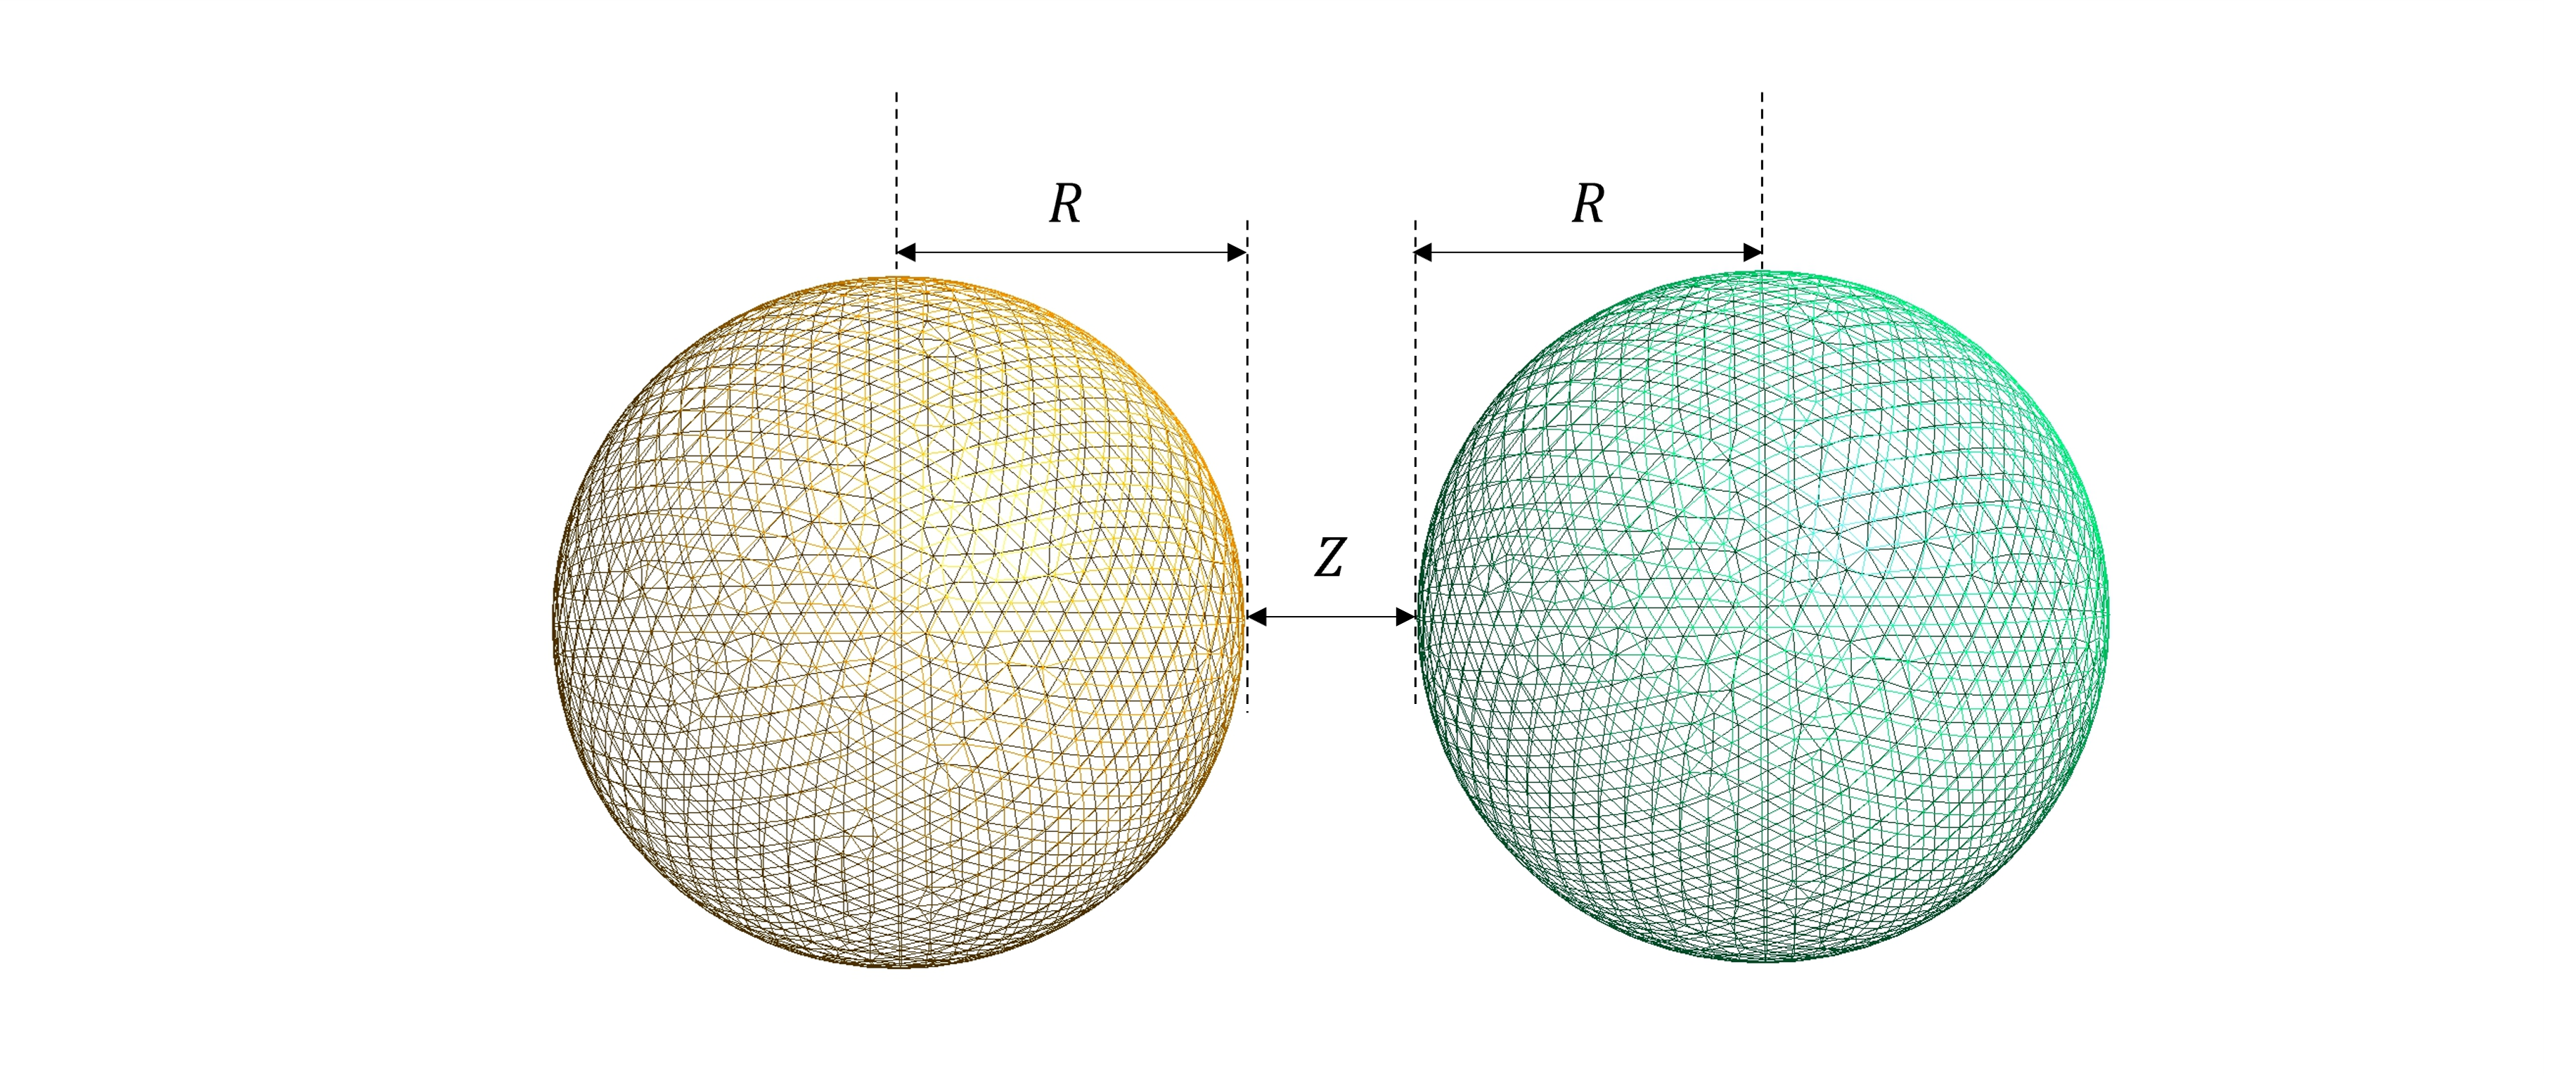
\includegraphics[scale = 0.6]{figures/Grid_two_spheres_dist.png}
    \caption{Two spheres with equal radii: $R$ represents the radius of the spheres and $Z$ is the distance between them.}
    \label{Two spheres with equal radii}
\end{figure}

Consider two perfectly conducting spheres with equal radii, which is shown in the Figure \ref{Two spheres with equal radii}. Inside the figure, $R$ is the radius 
of the spheres and the distance between them is denoted as $Z$. We firstly estimate the Casimir energy between the spheres with radius $R = 1$ and distance $Z$ 
ranging from 0.5 to 3.0 by using the equation \eqref{KSSF and CasE} with grid size set as $h_{\text{fine}} = 0.05$ and $h_{\text{coarse}} = 0.1$. Afterwards,
the extrapolation result can be obtained by substituting these Casimir energy estimates into the formula \eqref{Richardson extrapolation}. This result would be 
regarded as the exact value of the Casimir energy and be used to compare with the estimates derived from the asymptotic series introduced below. 

According to \cite{emig2008casimir}, the Casimir energy between these spheres (with equal radii $R$) at asymptotically 
large separations can be obtained as a series in terms of the ratio of centre distance $L$ ($L = 2R + Z$) to sphere radius $R$:
\begin{align}\label{Asymptotic equal radii}
   \mathcal{E} = -\frac{\hbar c}{\pi}\frac{1}{L}\sum_{n=0}^{\infty}b_{n}\left(\frac{R}{L}\right)^{n+2},
\end{align}
where the first six coefficients are 
$b_{0} = -1/4$, $b_{1} = -1/4$,  $b_{2} = -77/48$,  $b_{3} = -25/16$,  $b_{4} = -29837/2880$, $b_{5} = -6491/1152$. The value of Casimir energy computed from the 
asymptotic series \eqref{Asymptotic equal radii} is compared with the exact value evaluated through \eqref{KSSF and CasE} in Figure 
\ref{Casimir energy between spheres with equal radii}. In this figure, the asymptotic value gradually approaches to the exact value as the distance between the 
spheres increases since the asymptotic expansion \eqref{Asymptotic equal radii} only works when the distance between two spheres is asymptotically large.

\begin{figure}[H]
    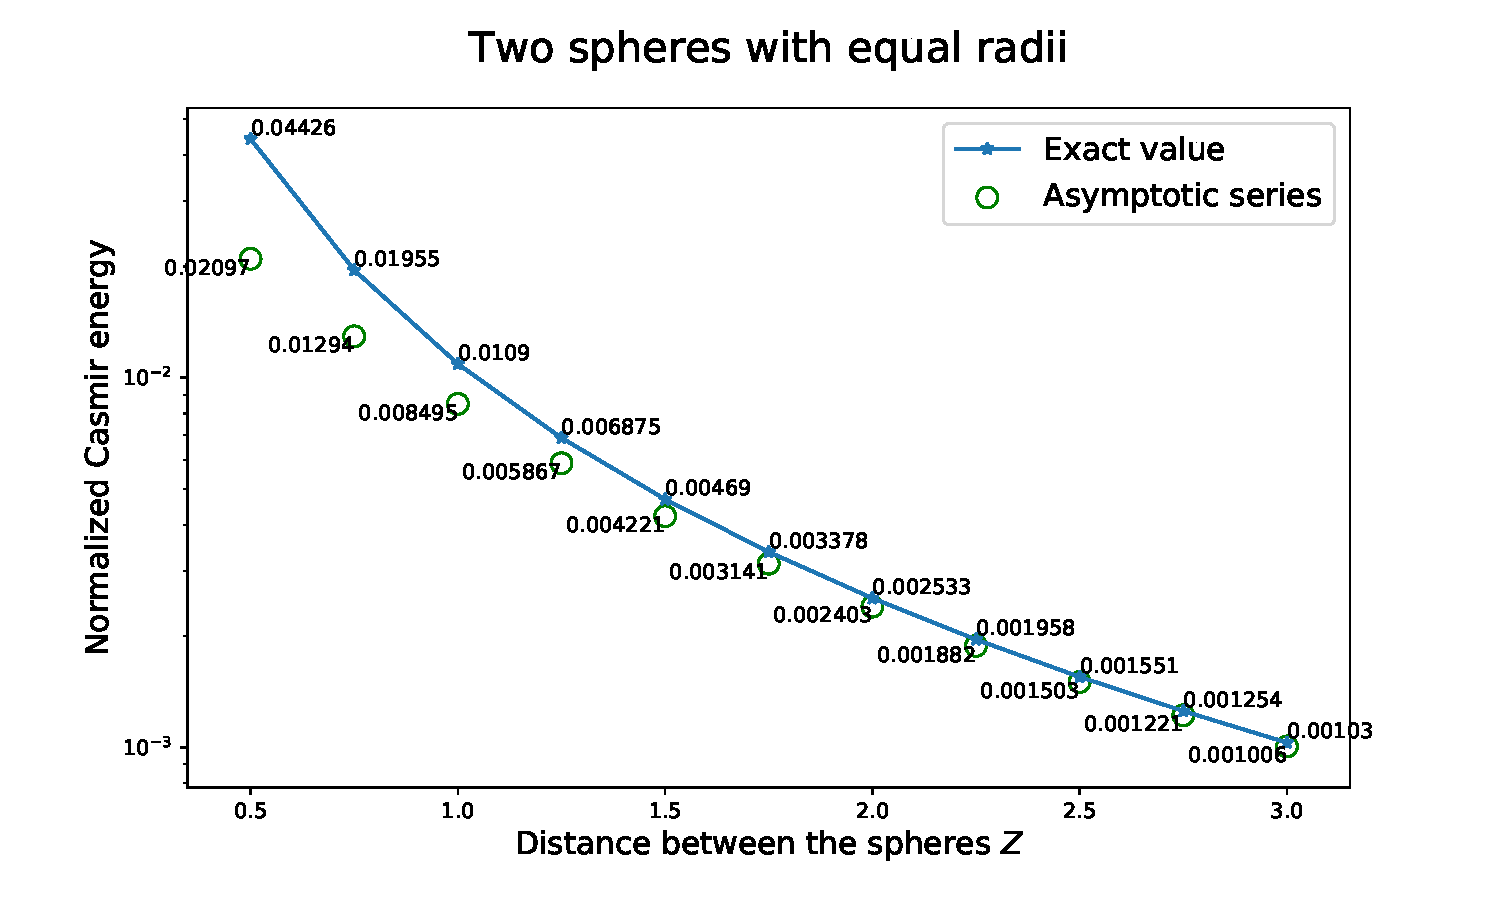
\includegraphics[scale = 0.7]{figures/Spheres_equal_CasE.pdf}
    \caption[Caption for LOF]{Normalized Casimir energy\protect\footnotemark in two spheres with equal radii's case. The exact value of the (normalized) Casimir 
    energy has been written beside the data point, which is round up to 4 significant digits.}
    \label{Casimir energy between spheres with equal radii}
\end{figure}
\footnotetext{The normalized Casimir energy is $\mathcal{E}/\hbar c$, for $\mathcal{E}$ defined in \eqref{KSSF and CasE}.}

Afterwards, in order to test the performance of the two efficient methods introduced in Section \ref{Krylov subspace for generalized eigenvalue problem}, we
would use them to evaluate the Casimir energy between two spheres described above. For the inverse-free Krylov subspace method, the dimension of the Krylov subspace is set as $m = 20$ and 50 and the 
number of approximated smallest (or largest) eigenvalues is $p = 10$ and 25, respectively. For the standard Arnoldi method, the dimension of the 
Krylov subspace is also set as $m = 20$ and 50. In Figure \ref{equal_radii_rel_dist}, we can easily find the inverse-free Krylov subspace method behaves better 
than the standard Arnoldi method no matter when the dimension $m$ is 20 or 50 and as we increase the Krylov subspace dimension, the relative distance decreases.
In addition, it can be noticed that when the distance $Z$ between the spheres increases, the relative error 
for both methods goes down. The reason is when the spheres are getting away from each other, the cross interaction between them becomes weaker and the compact 
perturbation $\tilde{\mathsf{V}}_{k}$ becomes close to $\mathsf{V}_{k}$, which implies the number of the eigenvalues that mainly contribute on the log 
determinant of $\mathsf{V}_{k}\tilde{\mathsf{V}}_{k}^{-1}$ decreases. Therefore, if we keep setting the same dimension of Krylov subspace when the spheres
are at a large distance, we would have a better approximation on the Casimir energy.


\begin{figure}[H]
    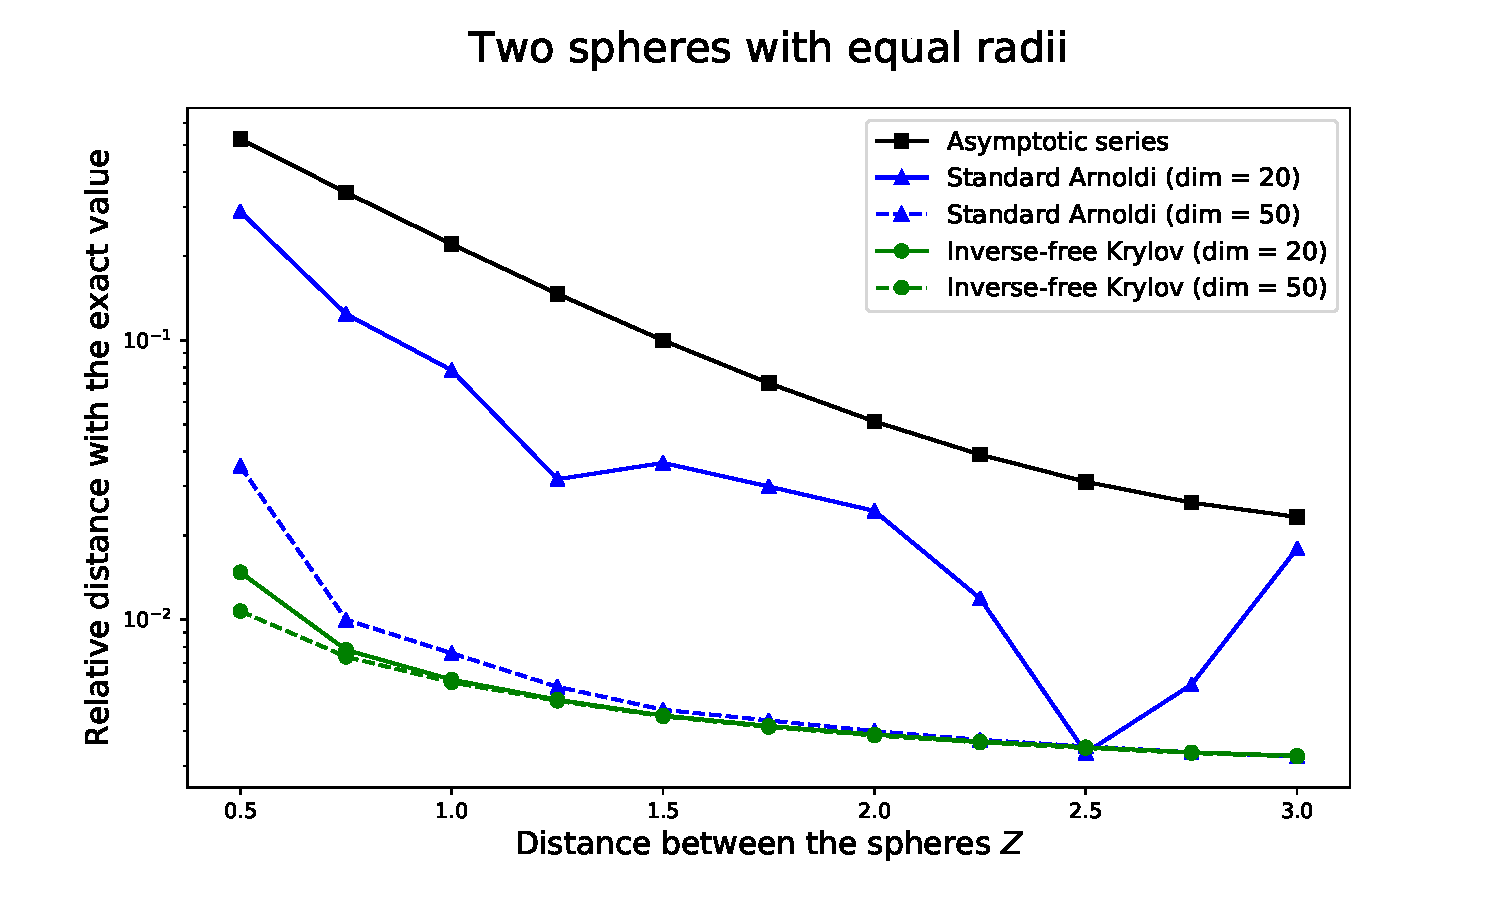
\includegraphics[scale = 0.7]{figures/relative_distance_equal_radii.pdf}
    \caption{Relative distance between the reference value (computed by Richardson extrapolation) with the asymptotic series and the estimates evaluated from 
    the standard Arnoldi method and inverse-free Krylov subspace method by setting the dimension of the Krylov subspace as $m = 20$ and 50 and for the inverse-free
    Krylov subspace method, the number of the approximated smallest (or largest) eigenvalues is set as $p = 10$ and 25, respectively.}
    \label{equal_radii_rel_dist}
\end{figure}
 
%================================================================================================================
\begin{figure}[H]
    \hspace*{2cm}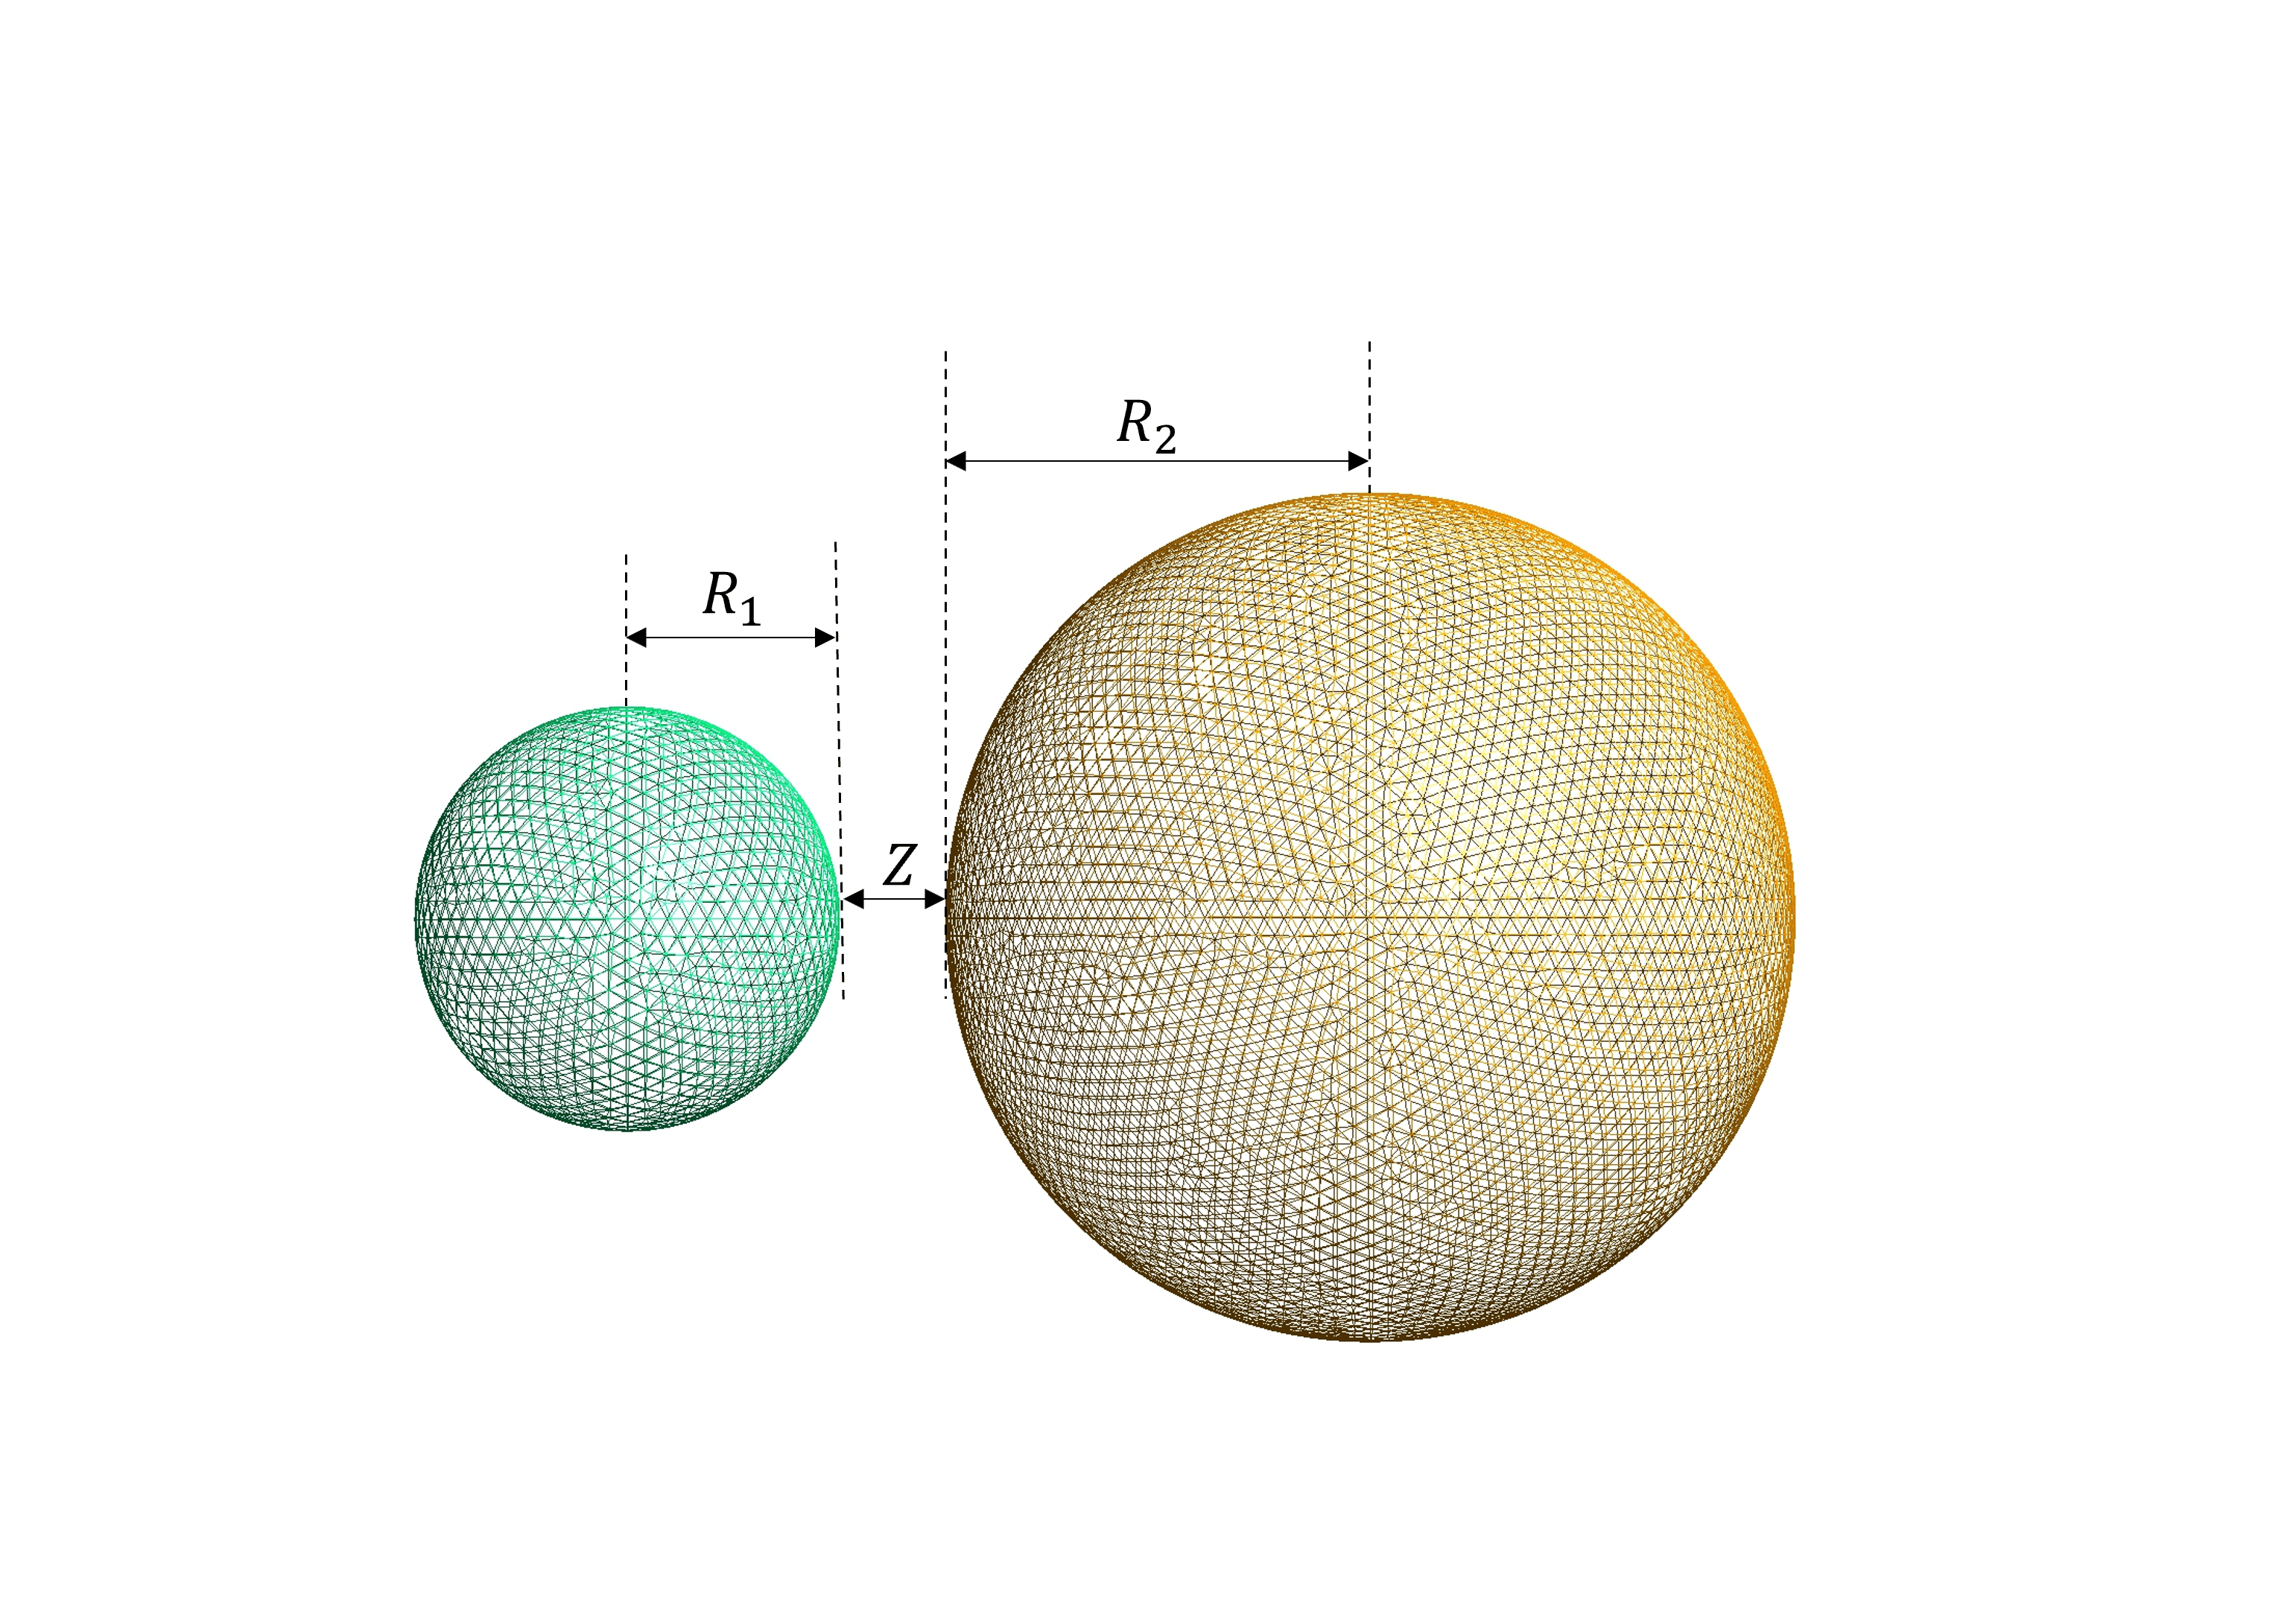
\includegraphics[scale = 0.6]{figures/Grid_two_spheres_unequal_radii.png}
    \caption{Two spheres with unequal radii: $R_{1}$ and $R_{2}$ represent the radius of the spheres and $Z$ is the distance between them.}
    \label{Two spheres with unequal radii}
\end{figure}

When the perfectly conducting spheres have different radii $R_{1}$, $R_{2}$ (see Figure \ref{Two spheres with unequal radii}) and the centre distance is denoted as
$L = R_{1} + R_{2} + Z$, the asymptotic expansion of the Casimir energy at asymptotically large distance can be written as:
\begin{align}\label{Asymptotic unequal radii}
    \mathcal{E} = -\frac{\hbar c}{\pi}\frac{1}{L}\sum_{n=0}^{\infty}\tilde{b}_{n}(\eta)\left(\frac{R_{1}}{L}\right)^{n+2},
\end{align}
where the coefficients $\{\tilde{b}_{n}\}$ depend on the parameter $\eta = R_{2}/R_{1}$ and the first six coefficients are
\begin{align*}
    \tilde{b}_{0} &= -\frac{\eta}{4}, \ \ \ \ \ \tilde{b}_{1} = -\frac{\eta + \eta^{2}}{8}, \ \ \ \ \  \tilde{b}_{2} = -\frac{34(\eta+\eta^{3})+ 9\eta^{2}}{48}, \ \ \ \ \ \tilde{b}_{3} = -\frac{2(\eta+\eta^{4}) + 23(\eta^{2} + \eta^{3})}{32}, \\ 
    \tilde{b}_{4} &= -\frac{8352(\eta + \eta^{5})+ 1995(\eta^{2} + \eta^{4}) + 38980\eta^{3}}{5760}, \ \ \ \ \ \tilde{b}_{5} = -\frac{-1344(\eta+\eta^{6}) + 5478(\eta^{2} + \eta^{5})+2357(\eta^{3} + \eta^{4})}{2304}.
\end{align*}

In the following experiment, the radii of the spheres shown in Figure \ref{Two spheres with unequal radii} are set as $R_{1} = 0.5$ and $ R_{2} = 1$. 
Afterwards, the exact value of the Casimir energy was computed through the Richardson extrapolation formula \eqref{Richardson extrapolation}, 
where the coarse and fine grid size are $h_{\text{coarse}} = 0.1$ and $h_{\text{fine}} = 0.05$, separately. The asymptotic value of the Casimir energy was 
estimated by the series \eqref{Asymptotic unequal radii} and the comparison between the exact value and asymptotic one is shown in Figure 
\ref{Casimir energy between spheres with unequal radii}. It can be noticed that when the distance between two spheres decreases, the asymptotic value gets 
close to the exact one and the reason for this is clearly stated in the above equal radii's case.
\begin{figure}[H]
    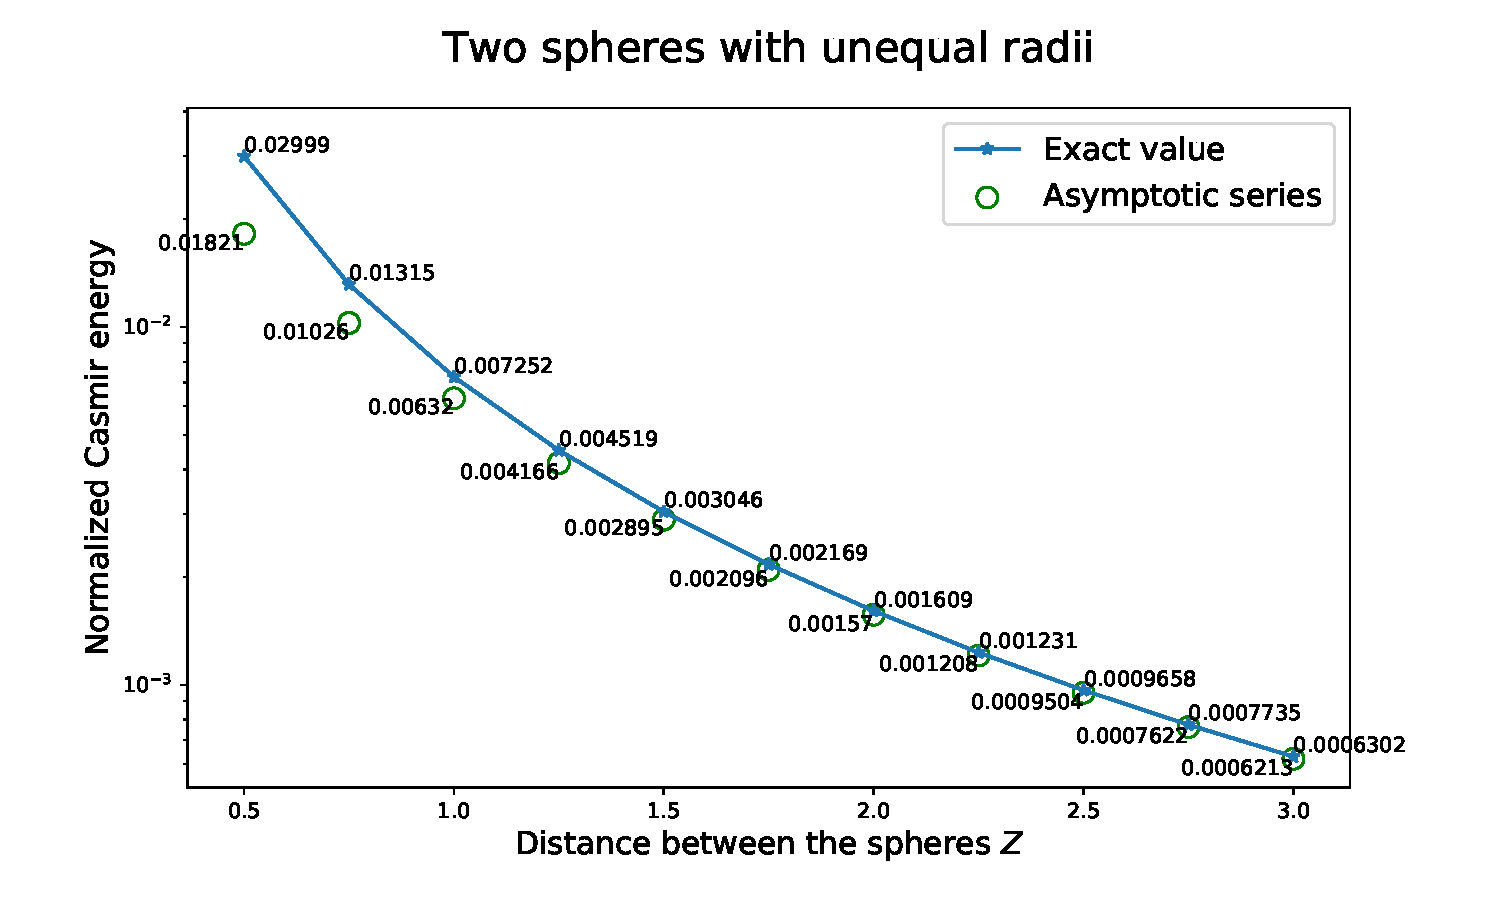
\includegraphics[scale = 0.7]{figures/Spheres_unequal_CasE.pdf}
    \caption{Normalized Casimir energy in two spheres with unequal radii's case. The exact value of the (normalized) Casimir energy has been written 
    beside the data point, which is round up to 4 significant digits.}
    \label{Casimir energy between spheres with unequal radii}
\end{figure}

By keeping all the experimental settings being the same with the equal radii's case, the experiment on testing the performance of the inverse-free and 
standard Arnoldi methods has been done in the unequal radii's case and the results are shown in Figure \ref{unequal_radii_rel_dist}. 
The main conclusion is similar to the previous case, that is the relative distance between the exact one and the estimate decreases when the distance between 
the spheres are getting away from each other. 

\begin{figure}[H]
    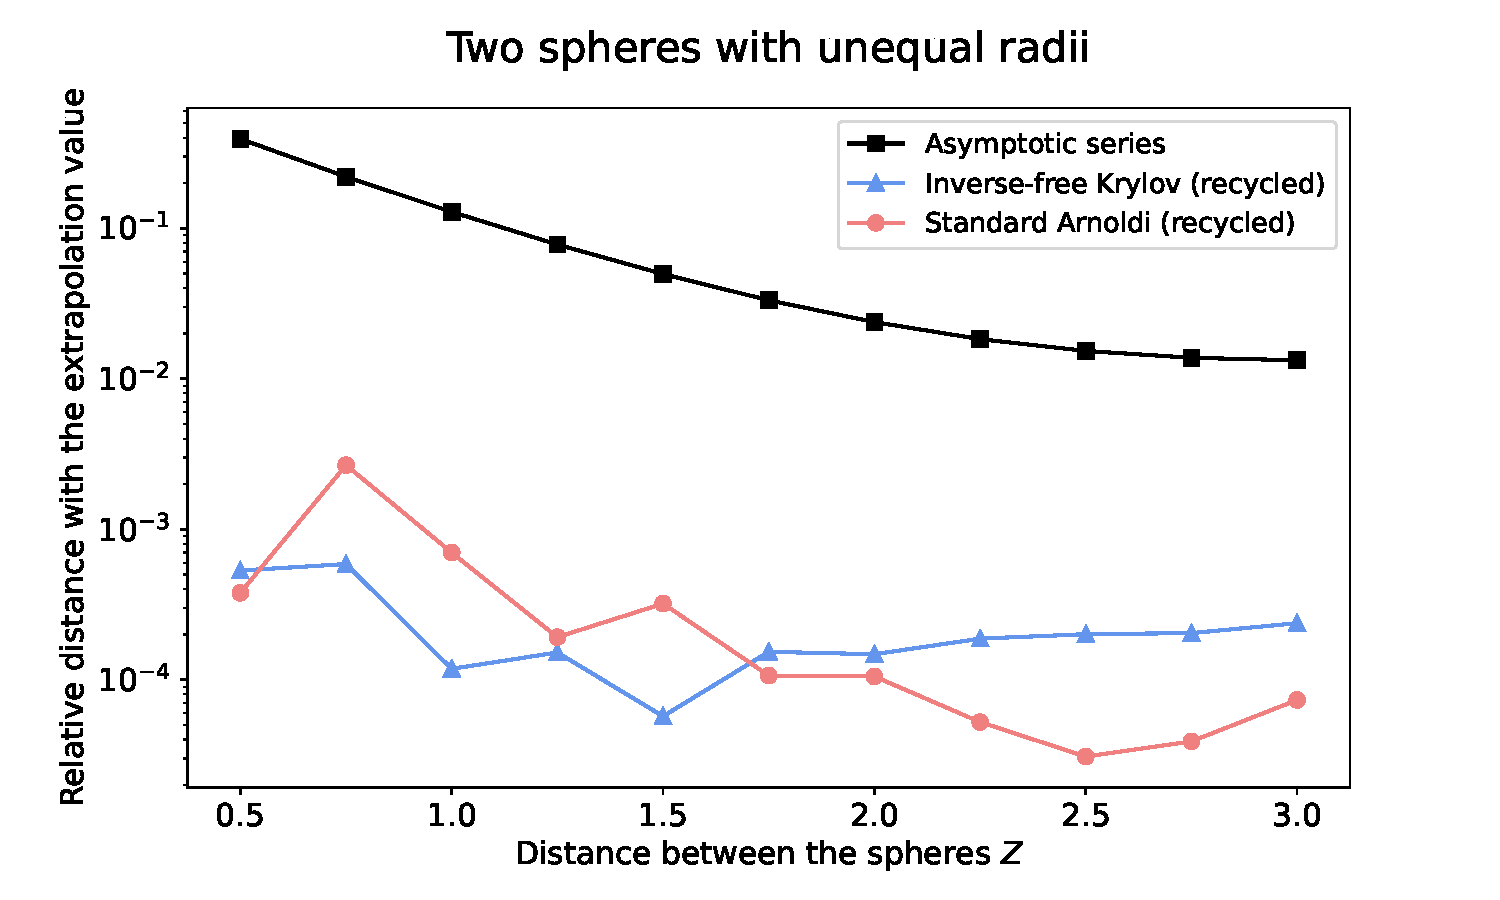
\includegraphics[scale = 0.7]{figures/relative_distance_unequal_radii.pdf}
    \caption{Relative distance between the reference value (computed by Richardson extrapolation) with the asymptotic series and the estimates evaluated from 
    the standard Arnoldi method and inverse-free Krylov subspace method by setting the dimension of the Krylov subspace as $m = 20$ and 50 and for the inverse-free
    Krylov subspace method, the number of the approximated smallest (or largest) eigenvalues is set as $p = 10$ and 25, respectively.}
    \label{unequal_radii_rel_dist}
\end{figure}

\subsection{Realistic objects case}
In this part, the Casimir energy between the objects with special shapes such as the menger sponges, ice crystals and ellipsoids is computed and 
the values labelled in the following figures are always round up to 4 significant digits. 

Figure \ref{Menger sponges} plots the menger sponges in different levels $l = 0, 1, 2$ and the length of the level-0 sponge (cube) is 1. Afterwards, the Casimir 
energy between two menger sponges in the same level are plotted in Figure \ref{Normalized Casimir energy in two menger sponges' case}. By comparing the data 
point in these subfigures, it is easy to find that the Casimir energy decreases as the number of the iteration increases since the cross-sectional 
area gets smaller.

\begin{figure}[H]
    \centering
    \subfloat[Level 0]{{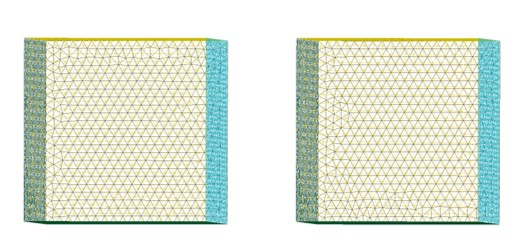
\includegraphics[width=0.4\textwidth]{figures/merger_sponge_level0.jpg} }}
    \qquad
    \subfloat[Level 1]{{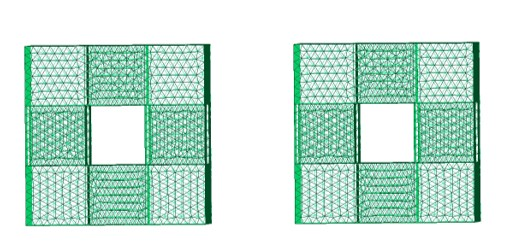
\includegraphics[width=0.4\textwidth]{figures/merger_sponge_level1.jpg} }}
    \qquad
    \subfloat[Level 2]{{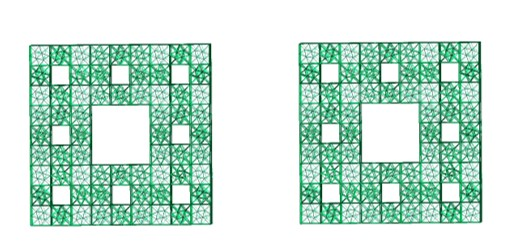
\includegraphics[width=0.4\textwidth]{figures/merger_sponge_level2.jpg} }}
    \caption{Menger sponges in different levels}
    \label{Menger sponges}
\end{figure}

\begin{figure}[H]
    \centering
    \hspace*{-1.5cm}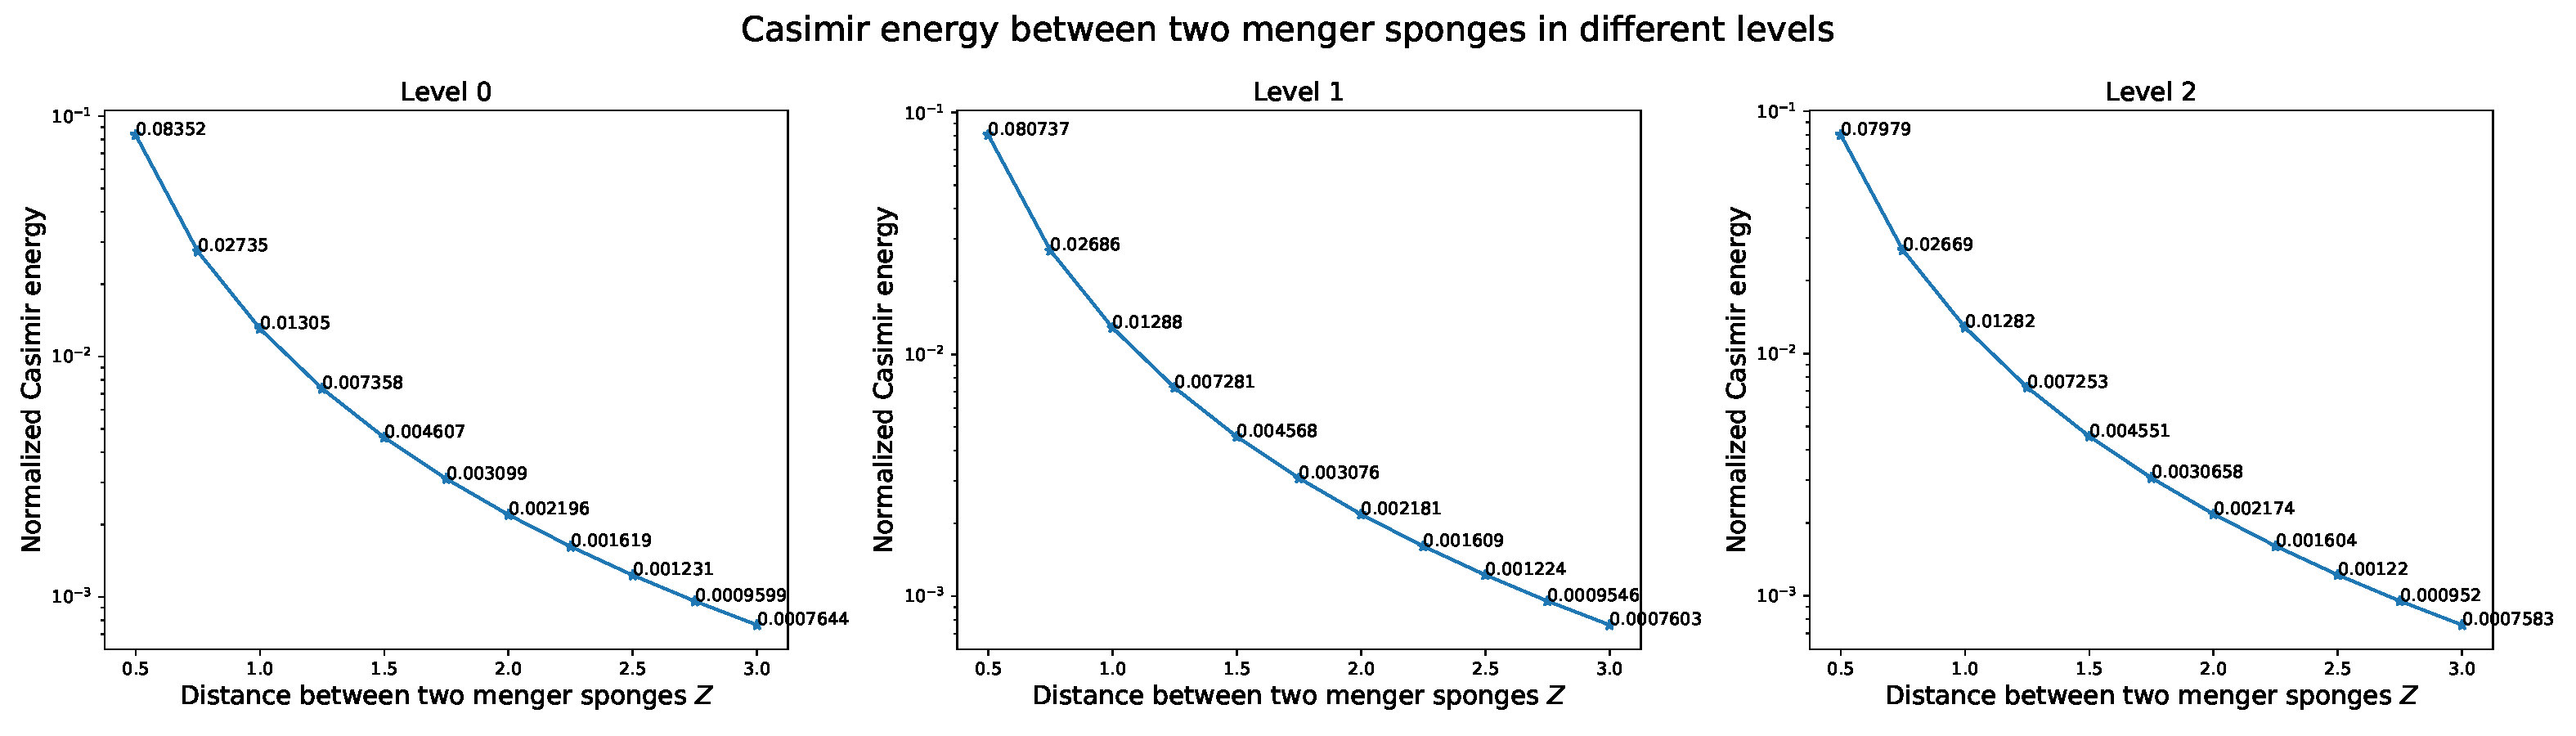
\includegraphics[width=1.2\textwidth]{figures/Cas_menger_spongers.pdf}
    \caption{Normalized Casimir energy in two menger sponges' case}
    \label{Normalized Casimir energy in two menger sponges' case}
\end{figure}
%==========================================================================================

\begin{figure}[H]
    \begin{subfigure}{0.3\linewidth}
        \centering
        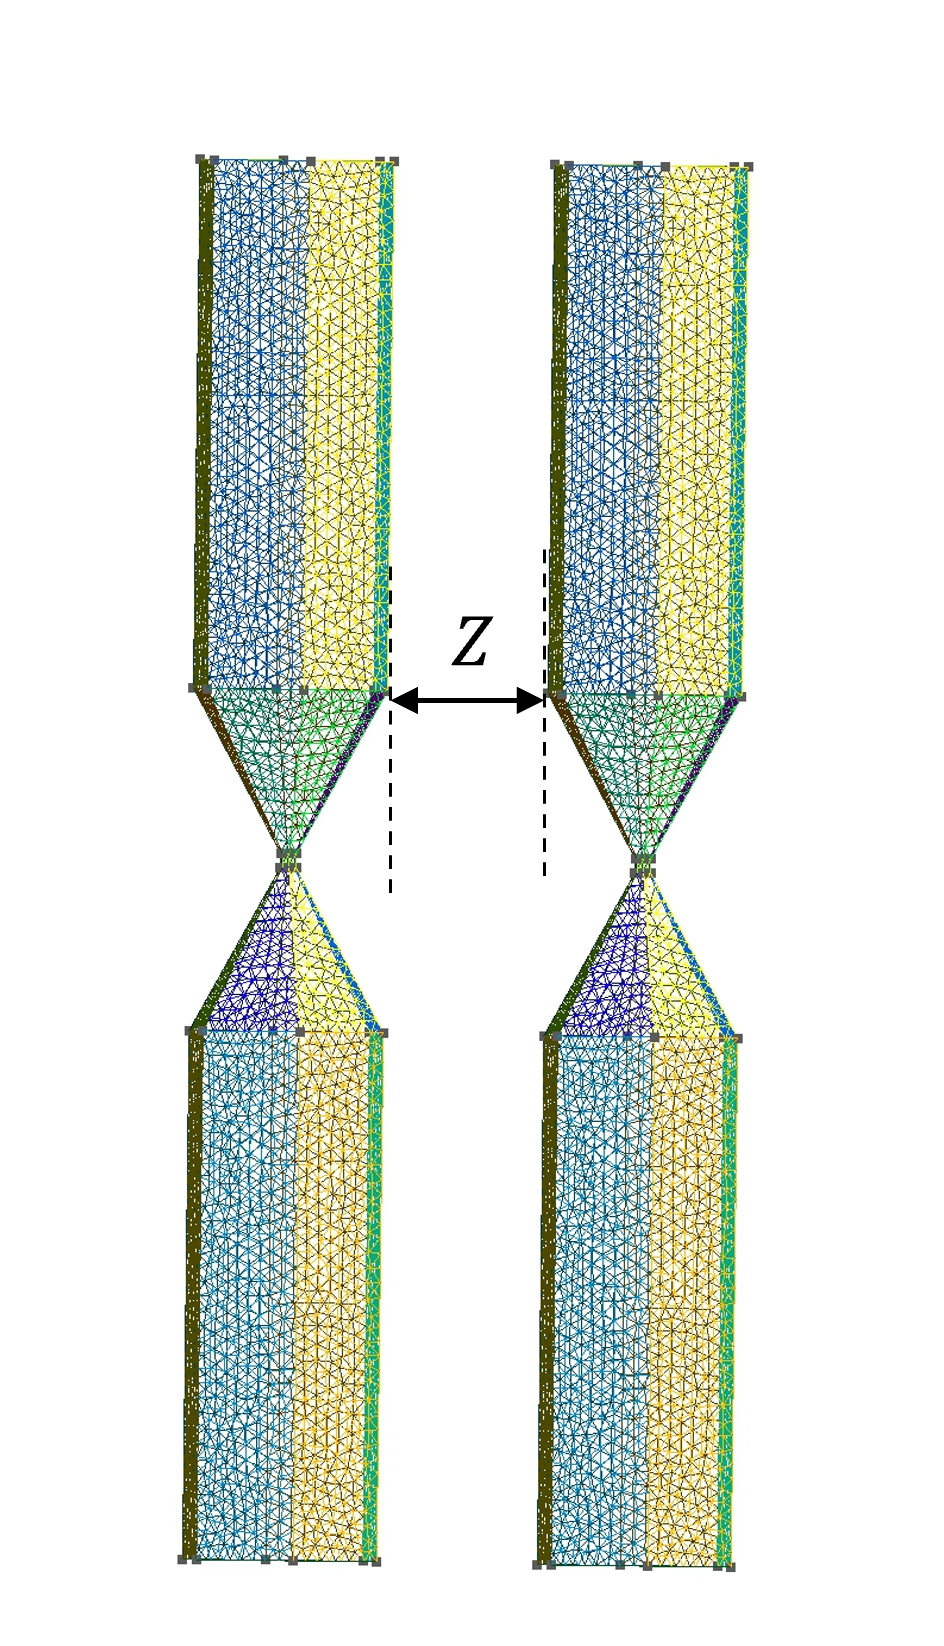
\includegraphics[scale = 0.4]{figures/2branches}
        \caption{Two branches}
        \end{subfigure}
        \begin{subfigure}{0.3\linewidth}
            \centering
            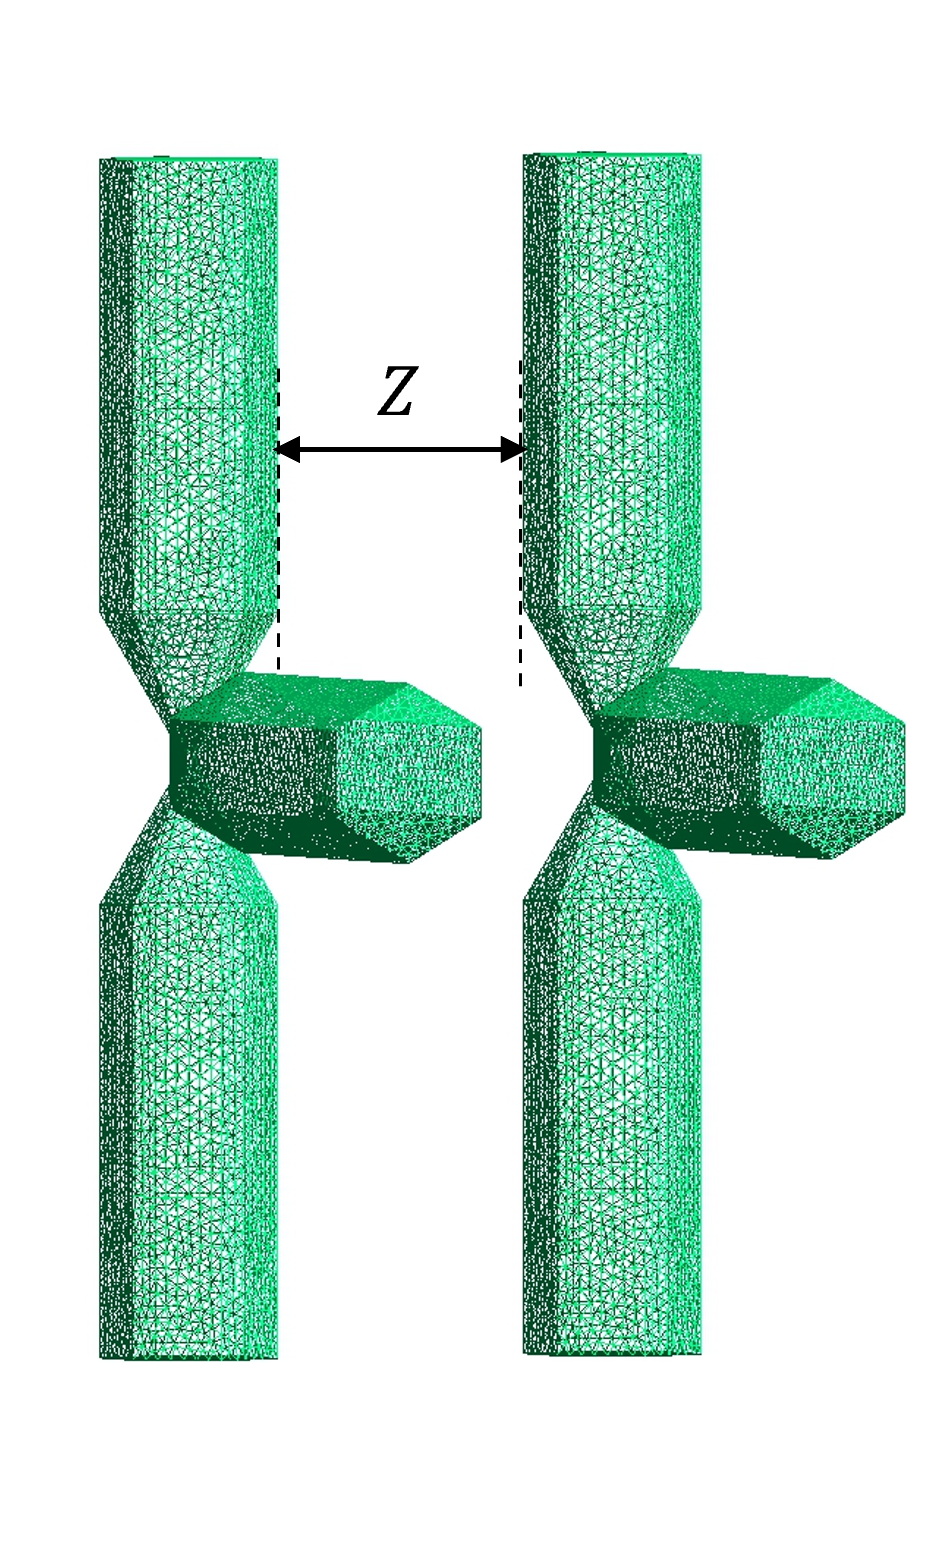
\includegraphics[scale = 0.4]{figures/3branches}
            \caption{Three branches}
            \end{subfigure}
            \begin{subfigure}{0.3\linewidth}
                \centering
                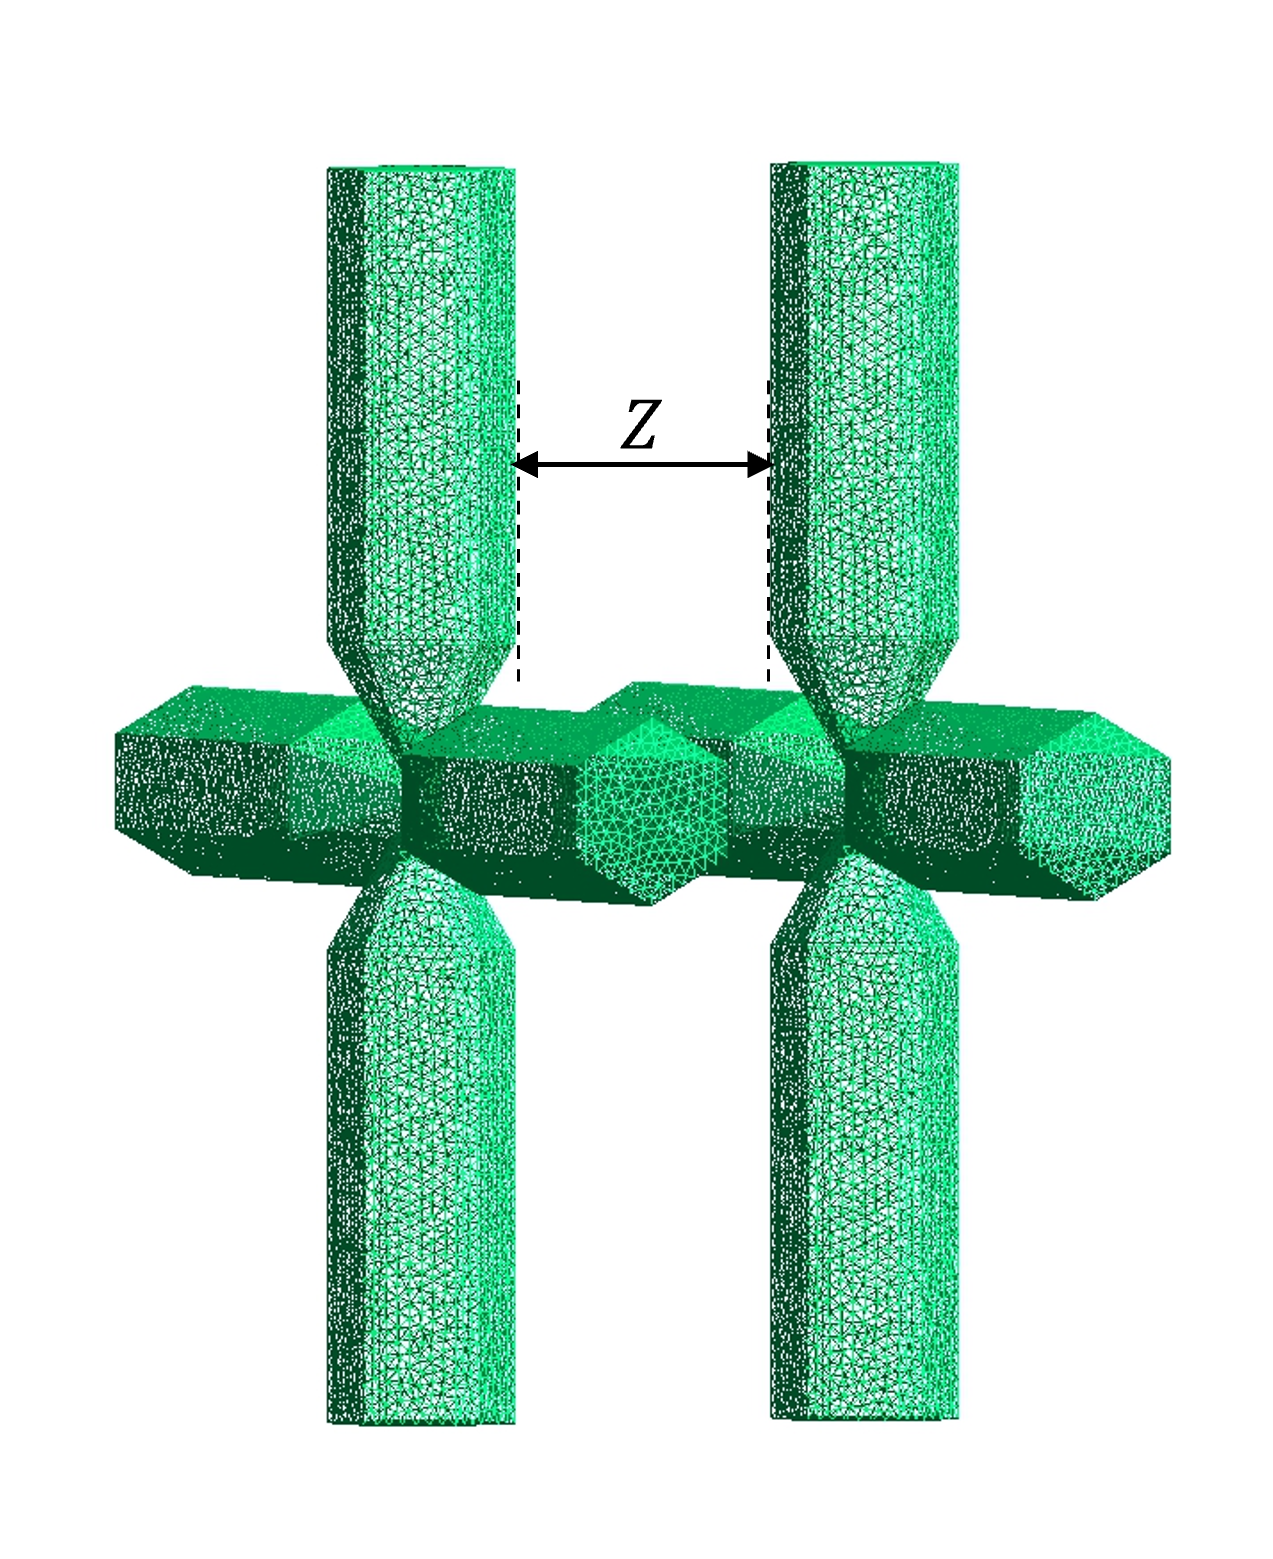
\includegraphics[scale = 0.38]{figures/4branches}
                \caption{Four branches}
                \end{subfigure}\\[1ex]
    \begin{subfigure}{.5\linewidth}
    \centering
    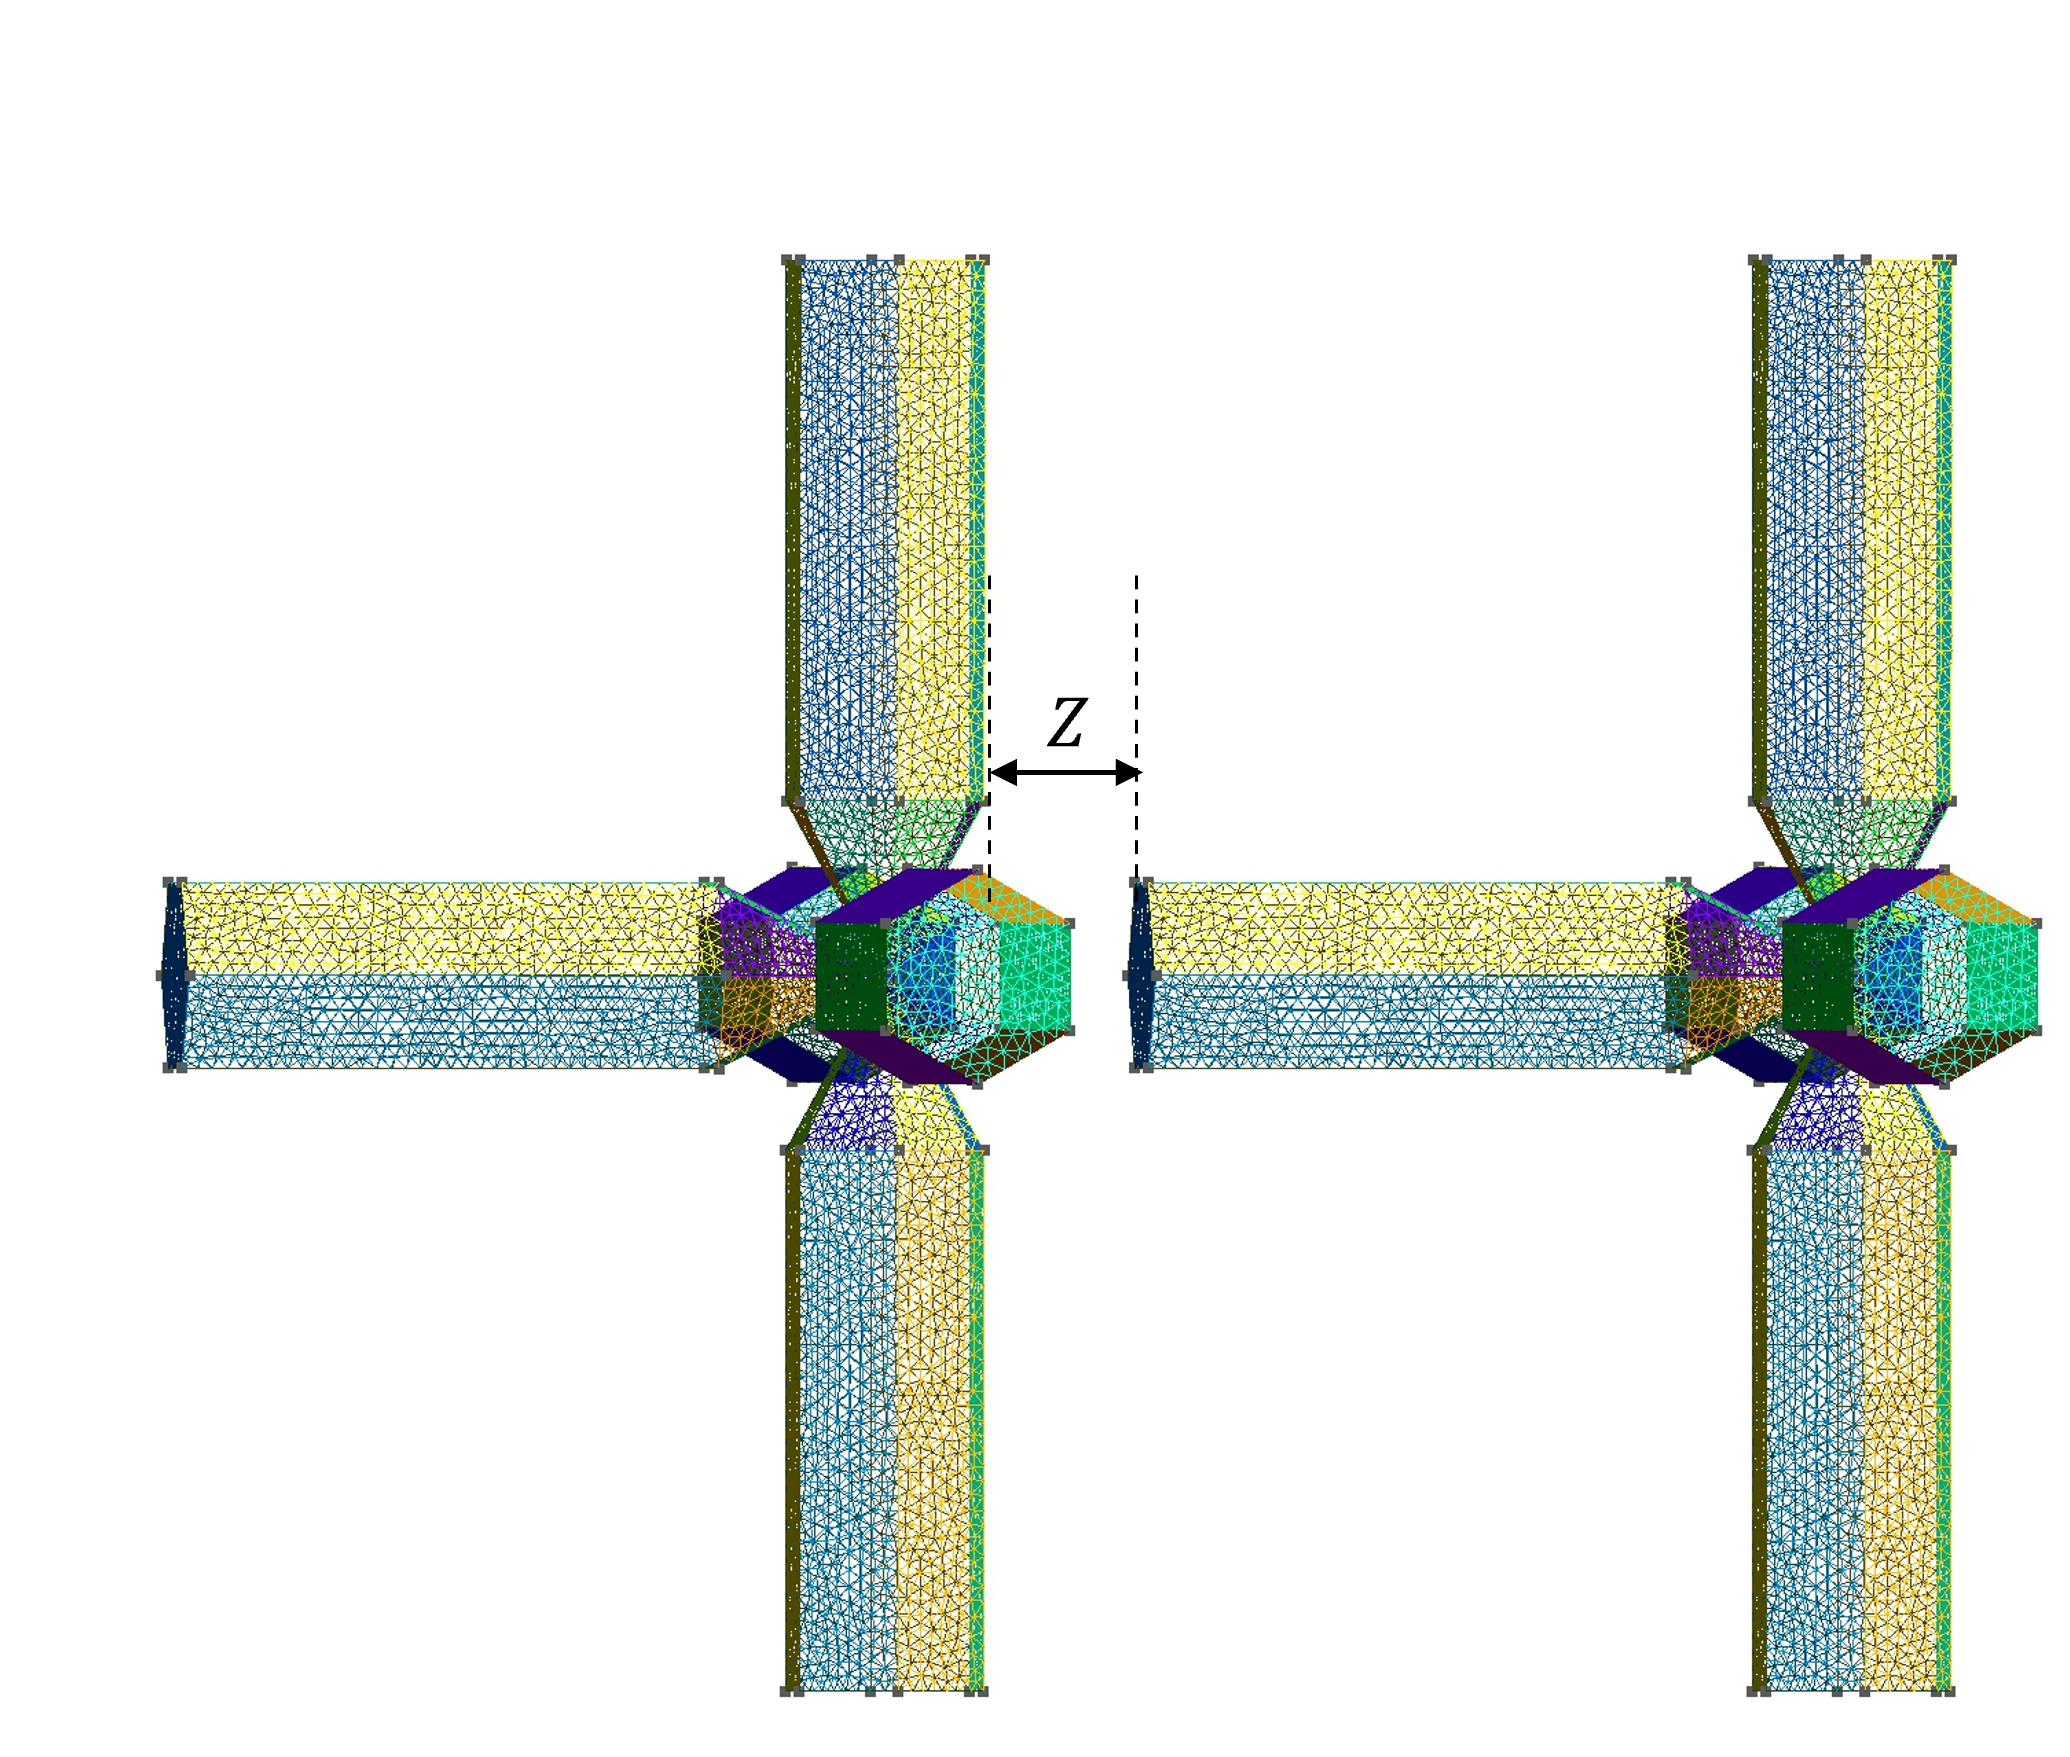
\includegraphics[scale = 0.4]{figures/5branches}
    \caption{Five branches}
    \end{subfigure}%
    \begin{subfigure}{.5\linewidth}
    \centering
    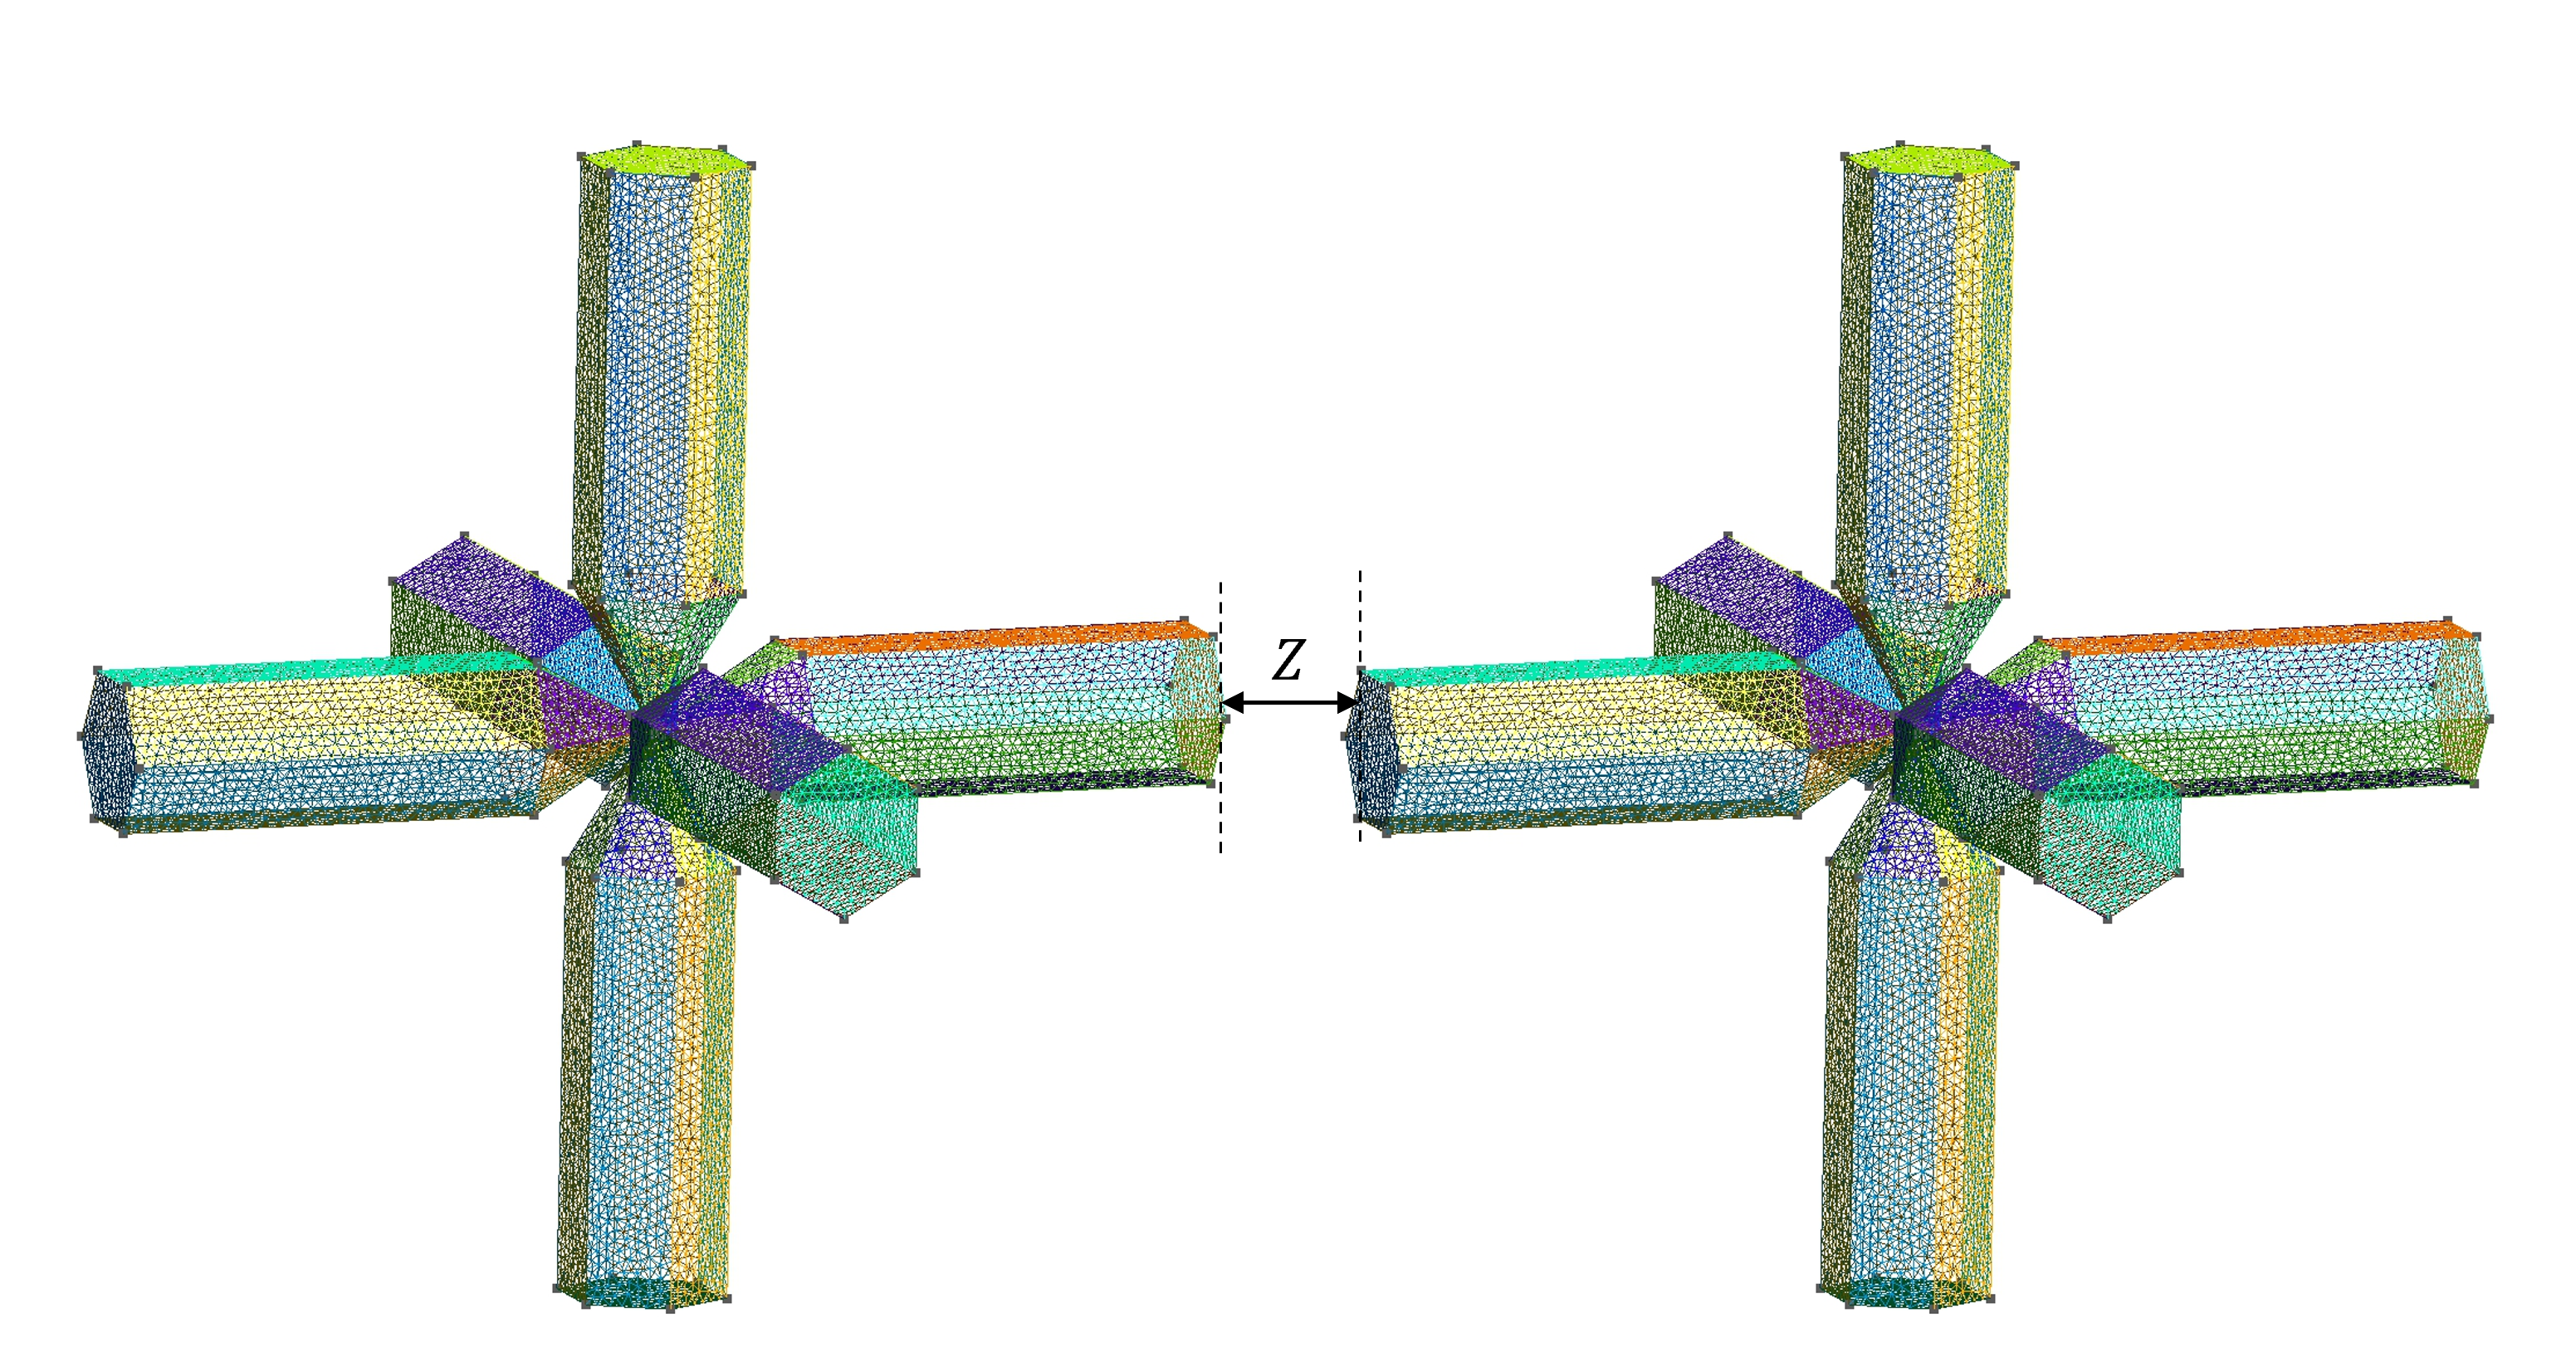
\includegraphics[scale = 0.4]{figures/6branches}
    \caption{Six branches}
    \end{subfigure}
    \caption{Ice crystals with different number of branches}
    \end{figure}

    \begin{figure}[H]
        \centering
        \hspace*{-1cm}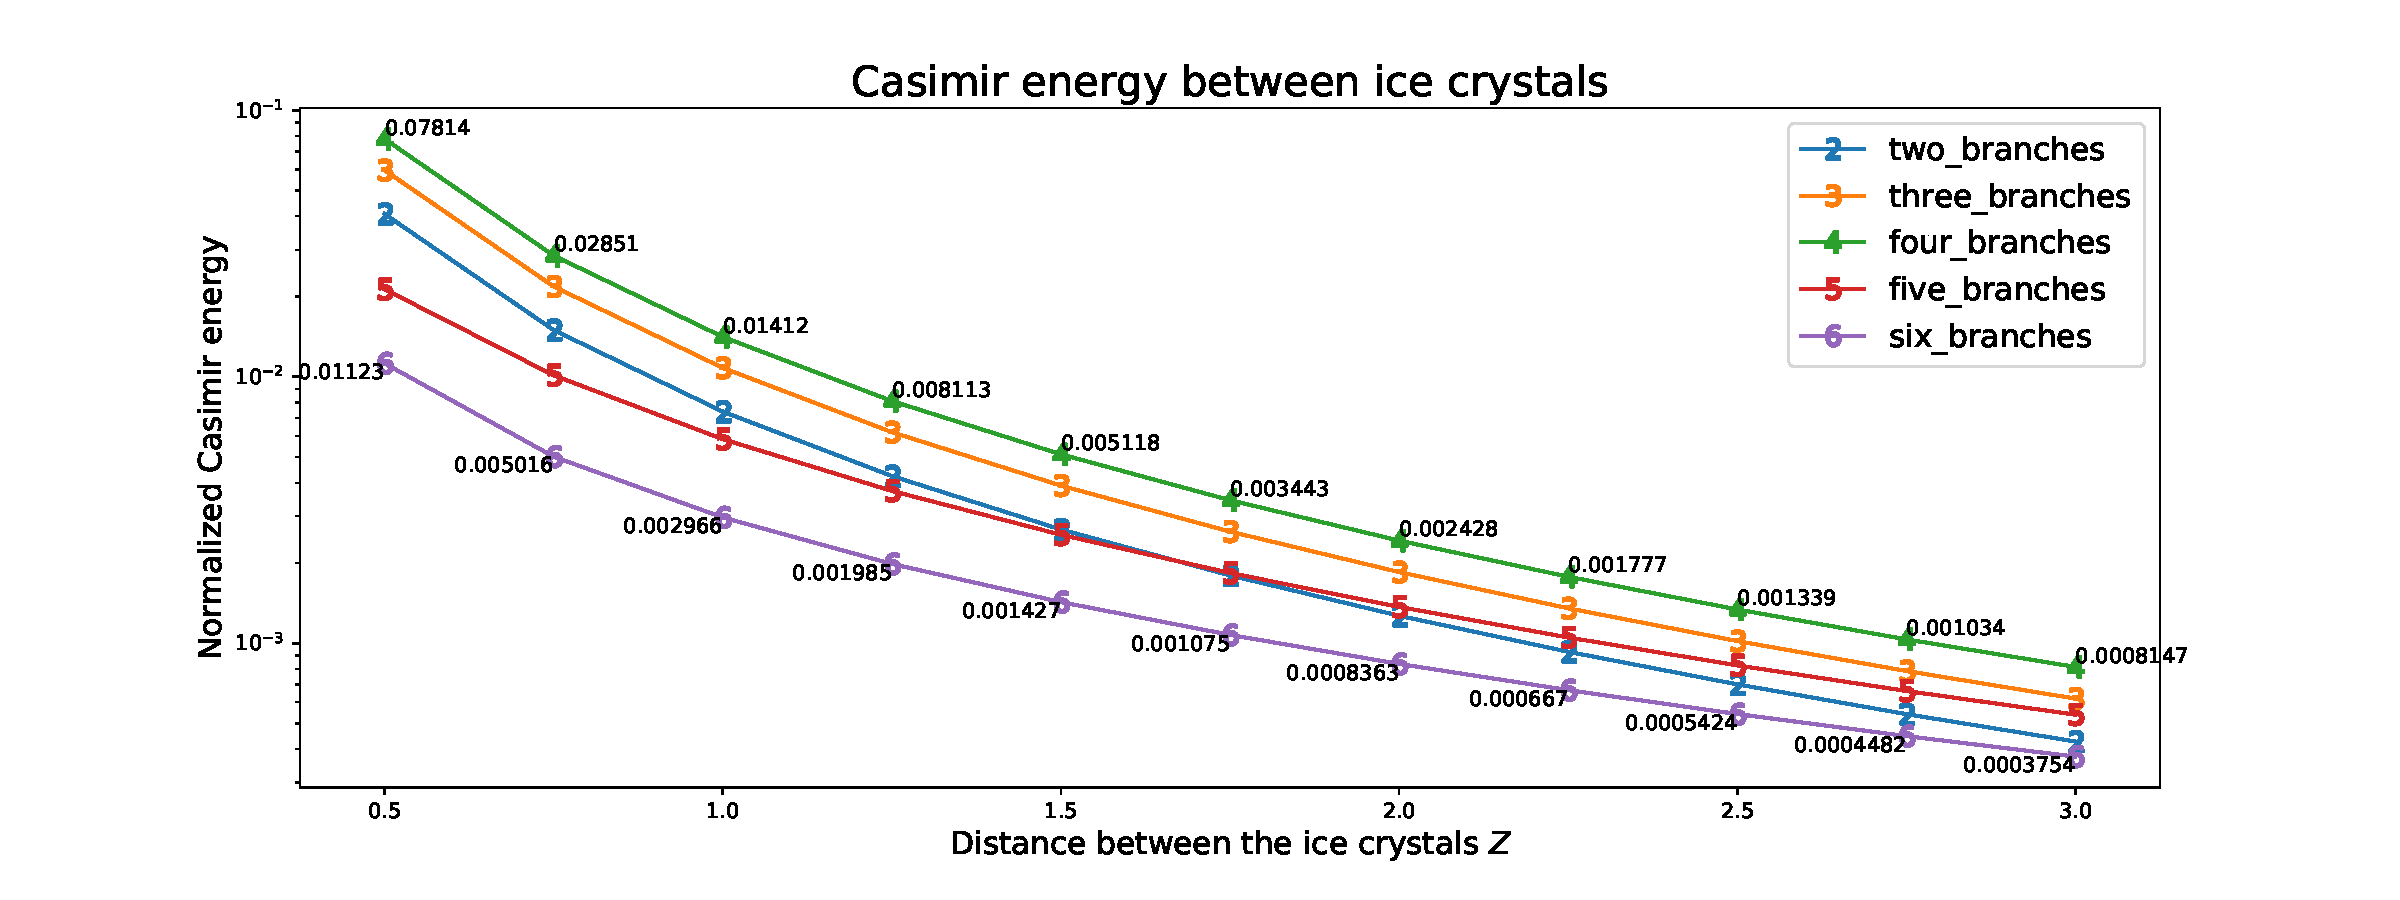
\includegraphics[scale = 0.5]{figures/CasE_ice_crystals.pdf}
        \caption{Casimir energy in ice crystals' case}
    \end{figure}
    

\begin{figure}[H]
    \begin{subfigure}{\linewidth}
        \centering
        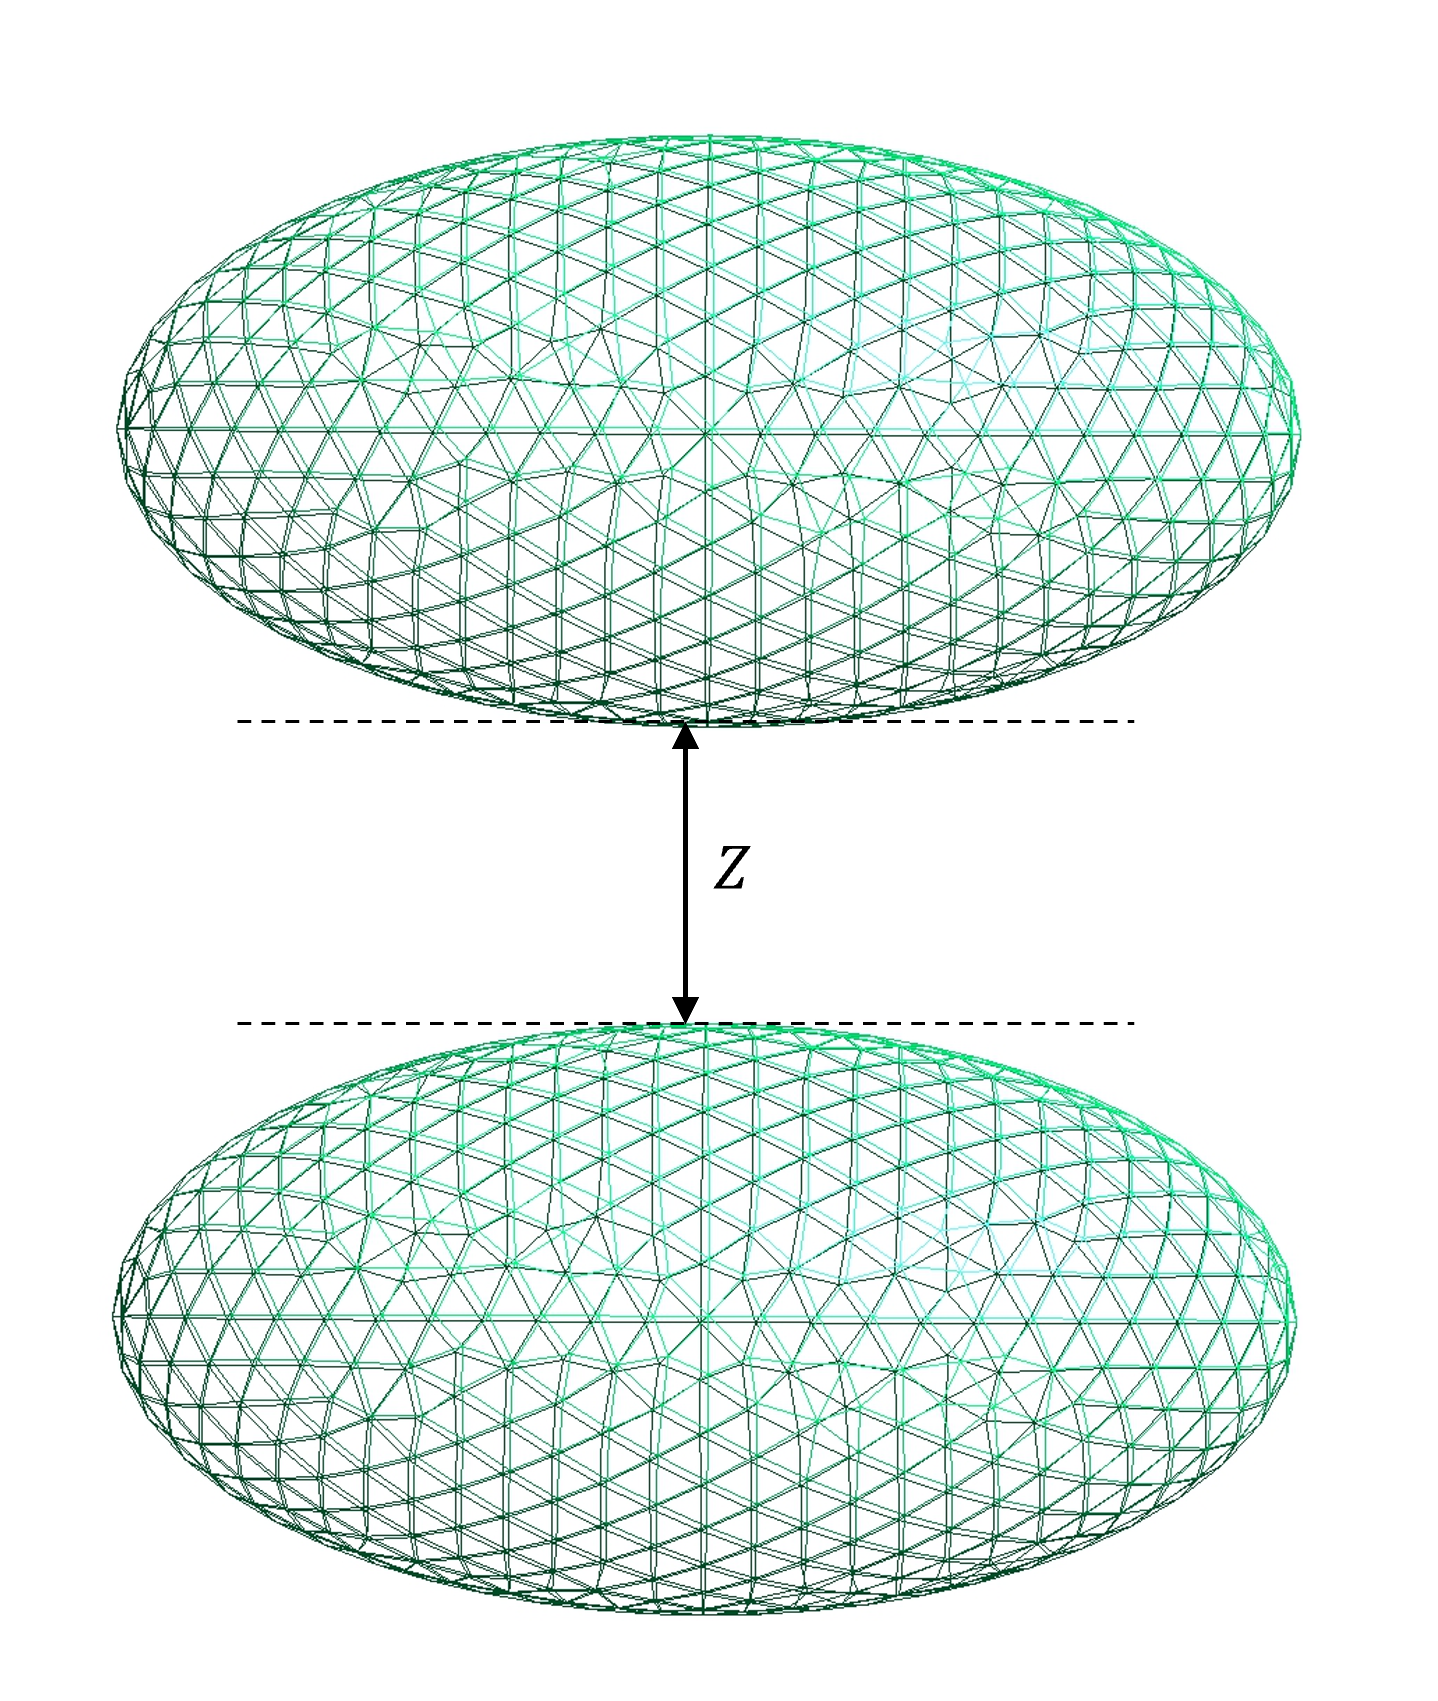
\includegraphics[scale = 0.4]{figures/two_ellipsoids}
        \caption{Without rotation}
        \end{subfigure}\\[1ex]
    \begin{subfigure}{.5\linewidth}
    \centering
    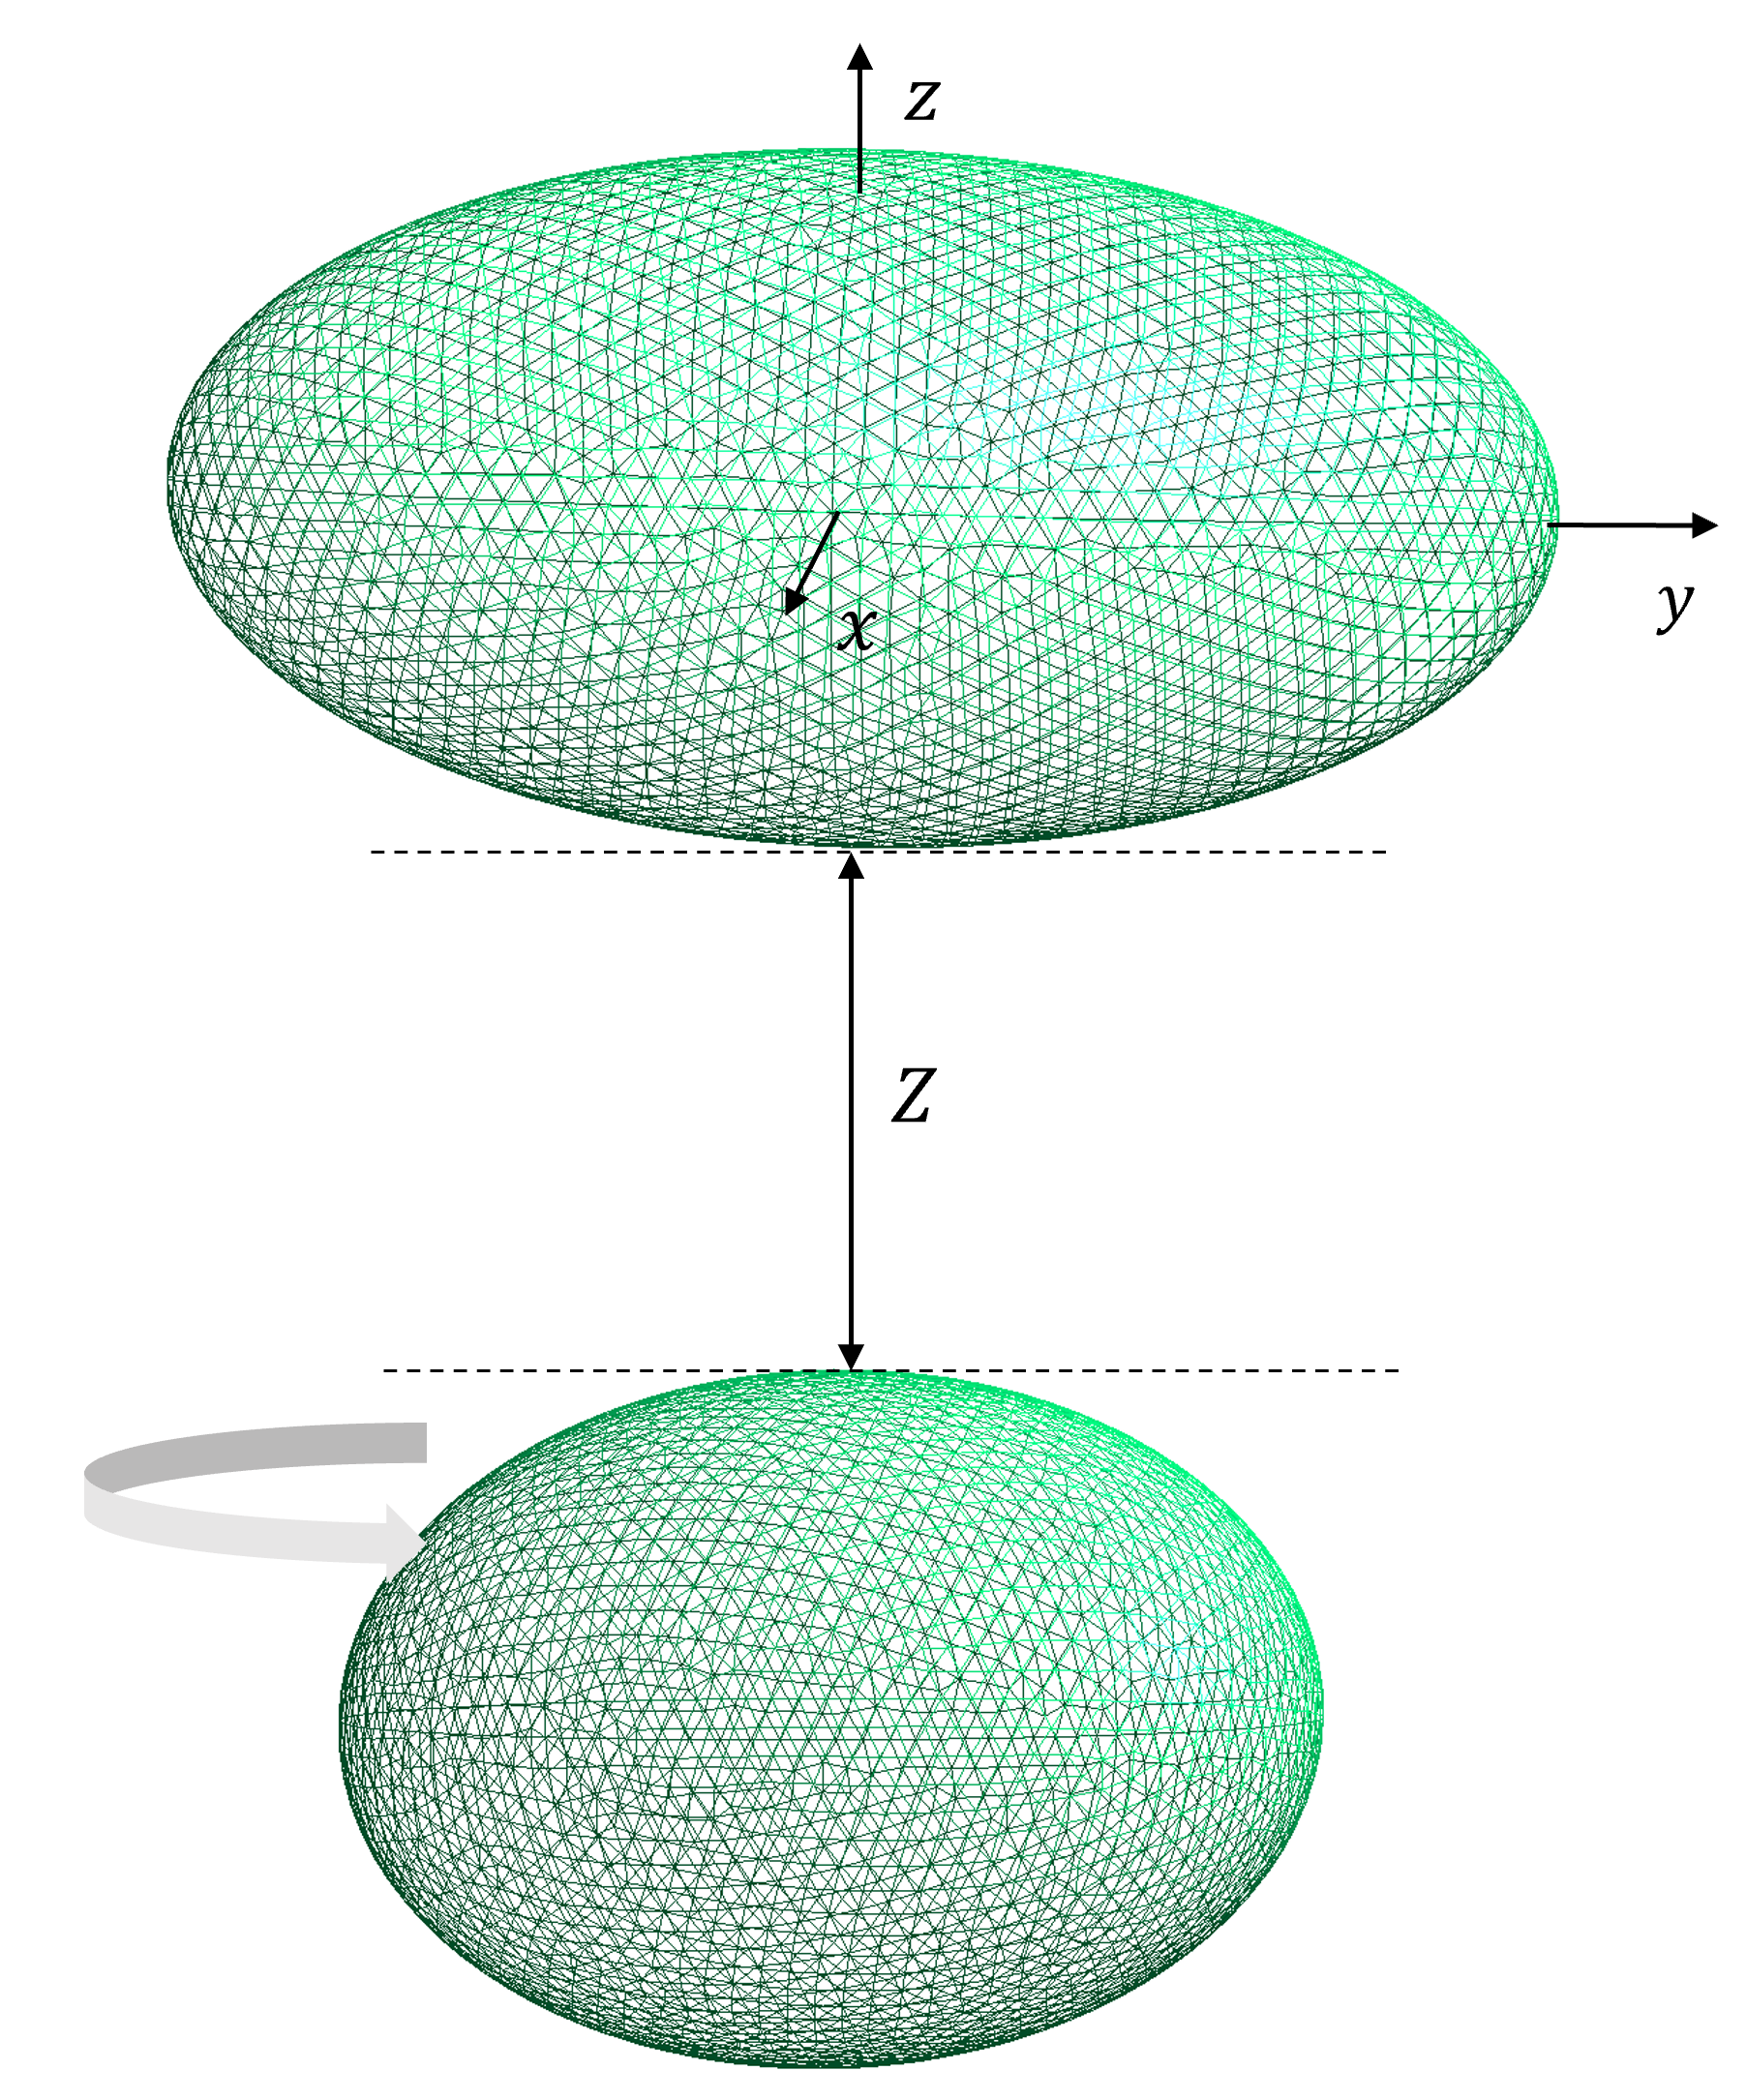
\includegraphics[scale = 0.4]{figures/Ellipsoid_z_axis}
    \caption{Rotation around z-axis}
    \end{subfigure}%
    \begin{subfigure}{.5\linewidth}
    \centering
    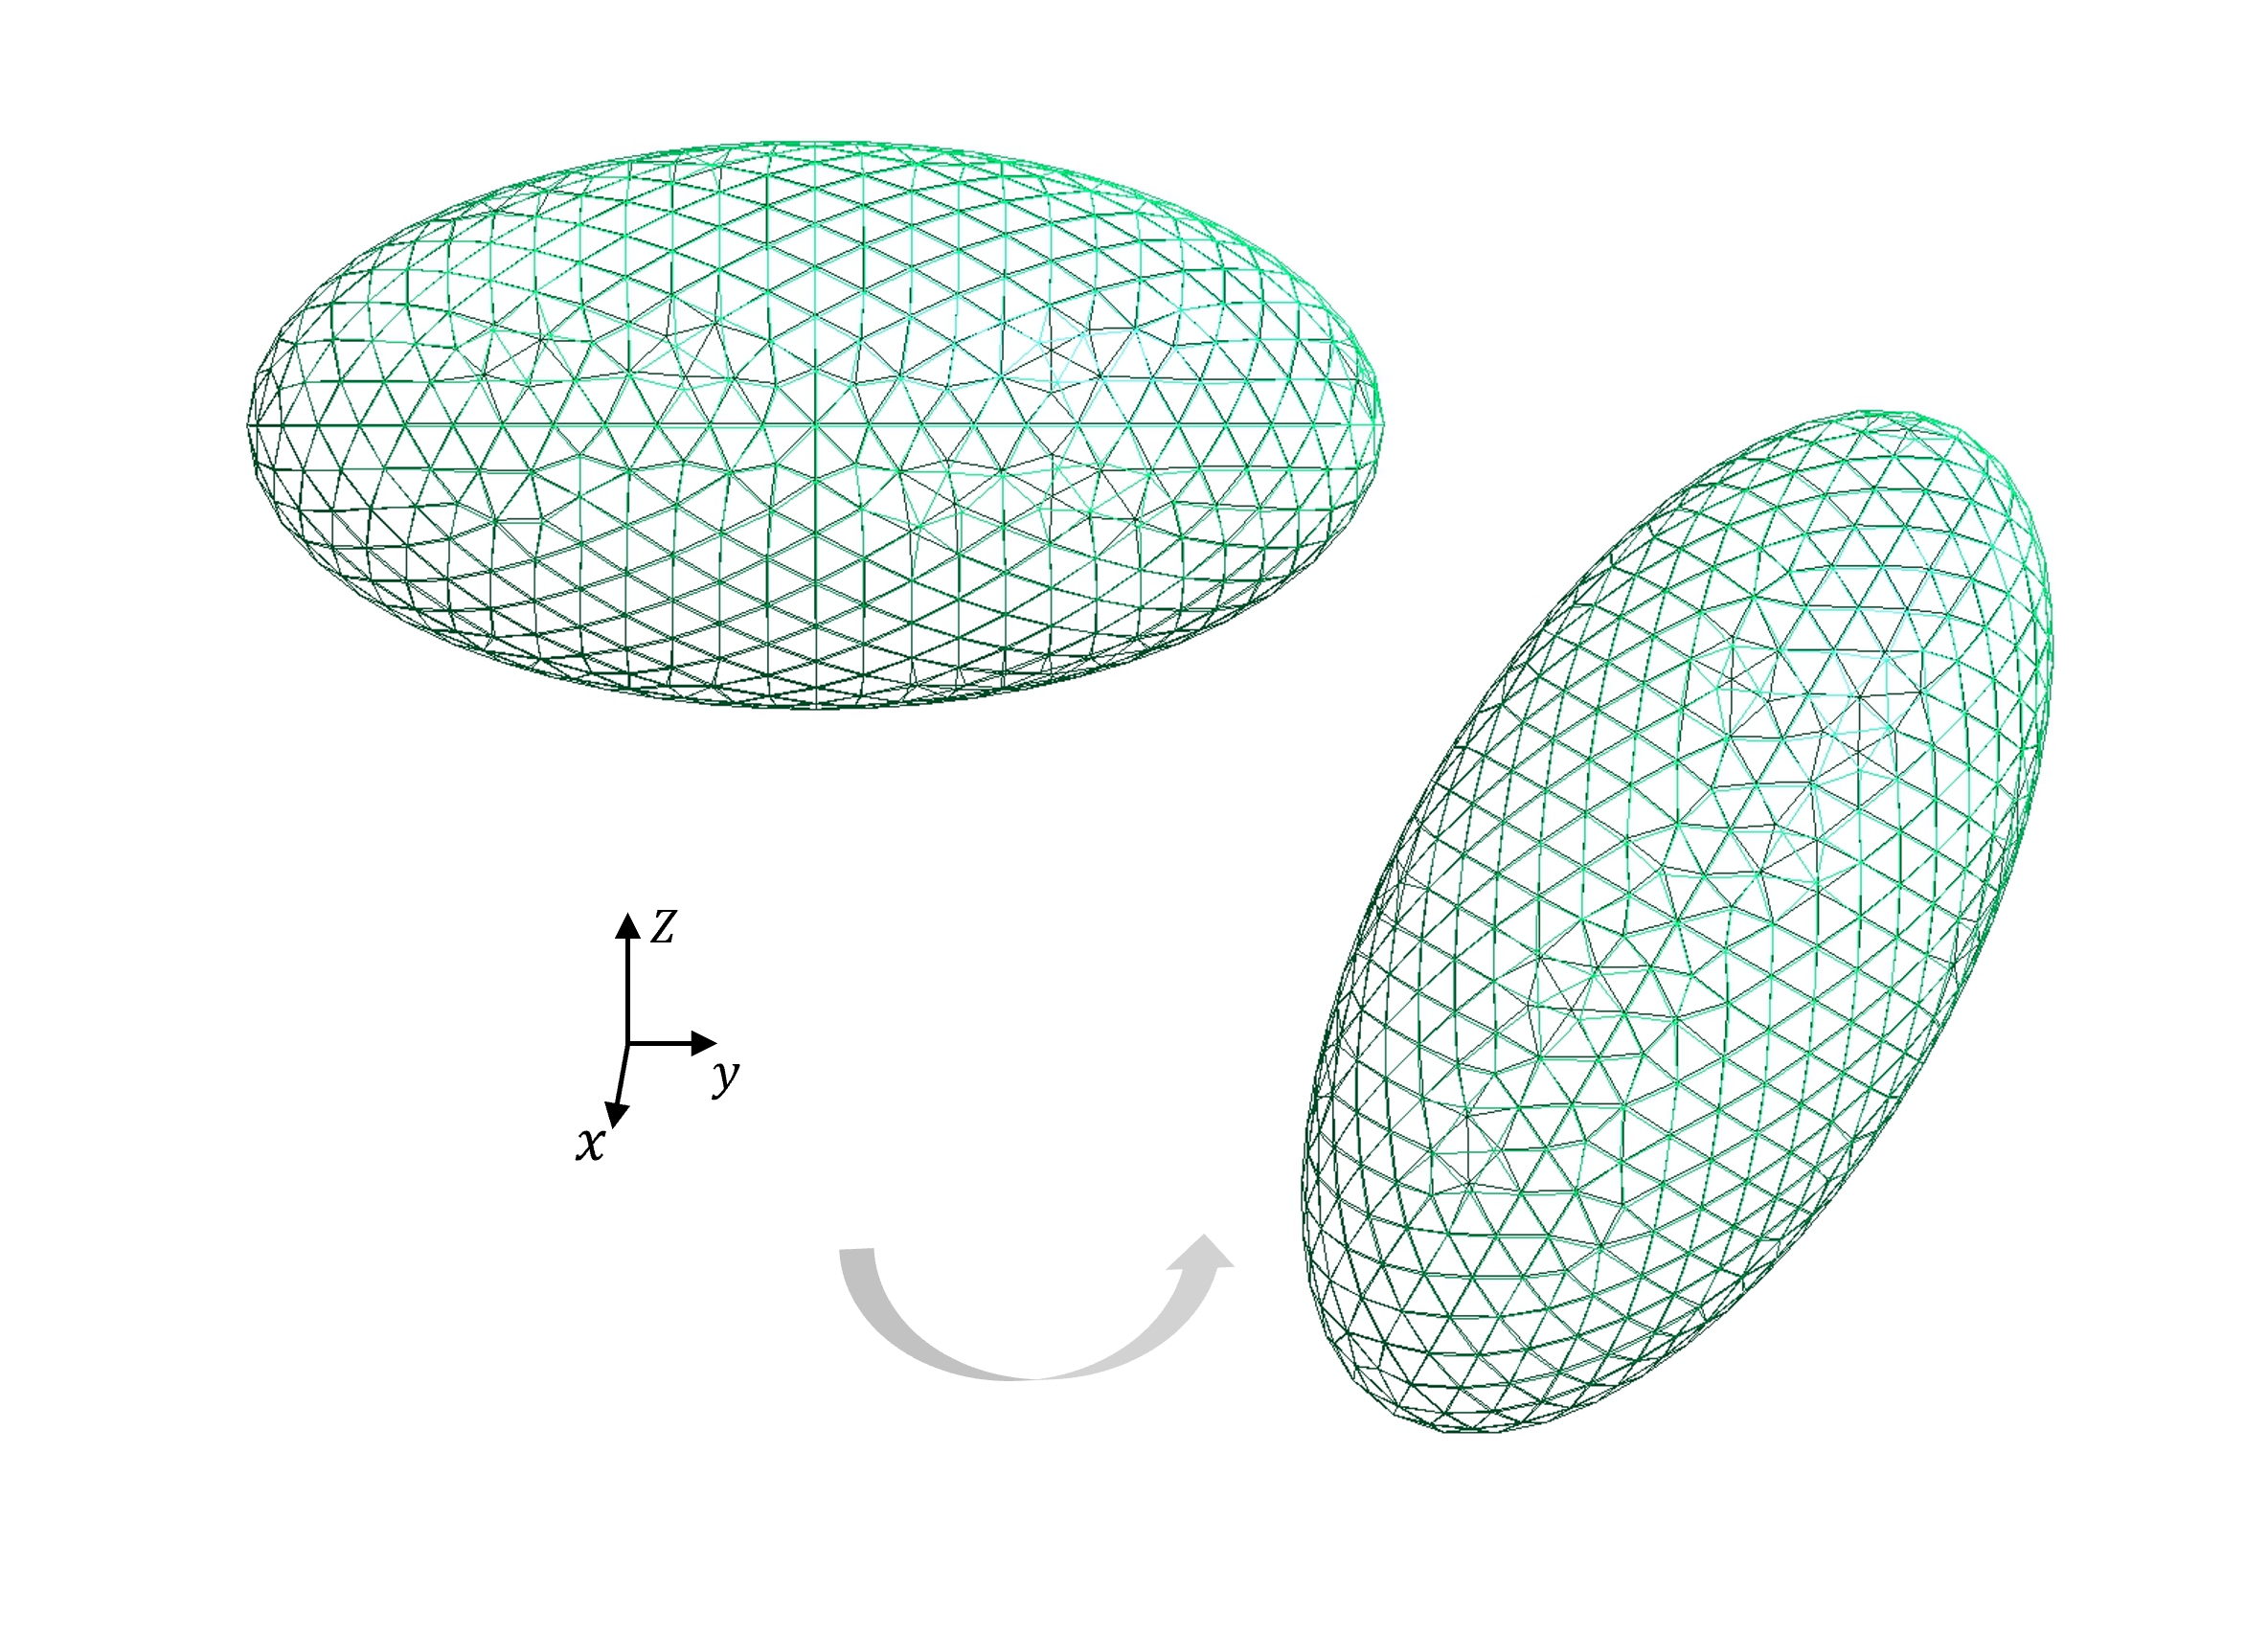
\includegraphics[scale = 0.4]{figures/Ellipsoid_x_axis}
    \caption{Rotation around x-axis}
    \end{subfigure}
    \caption{Two ellipsoids}
    \end{figure}

    \begin{figure}[H]
        \begin{subfigure}{\linewidth}
            \centering
            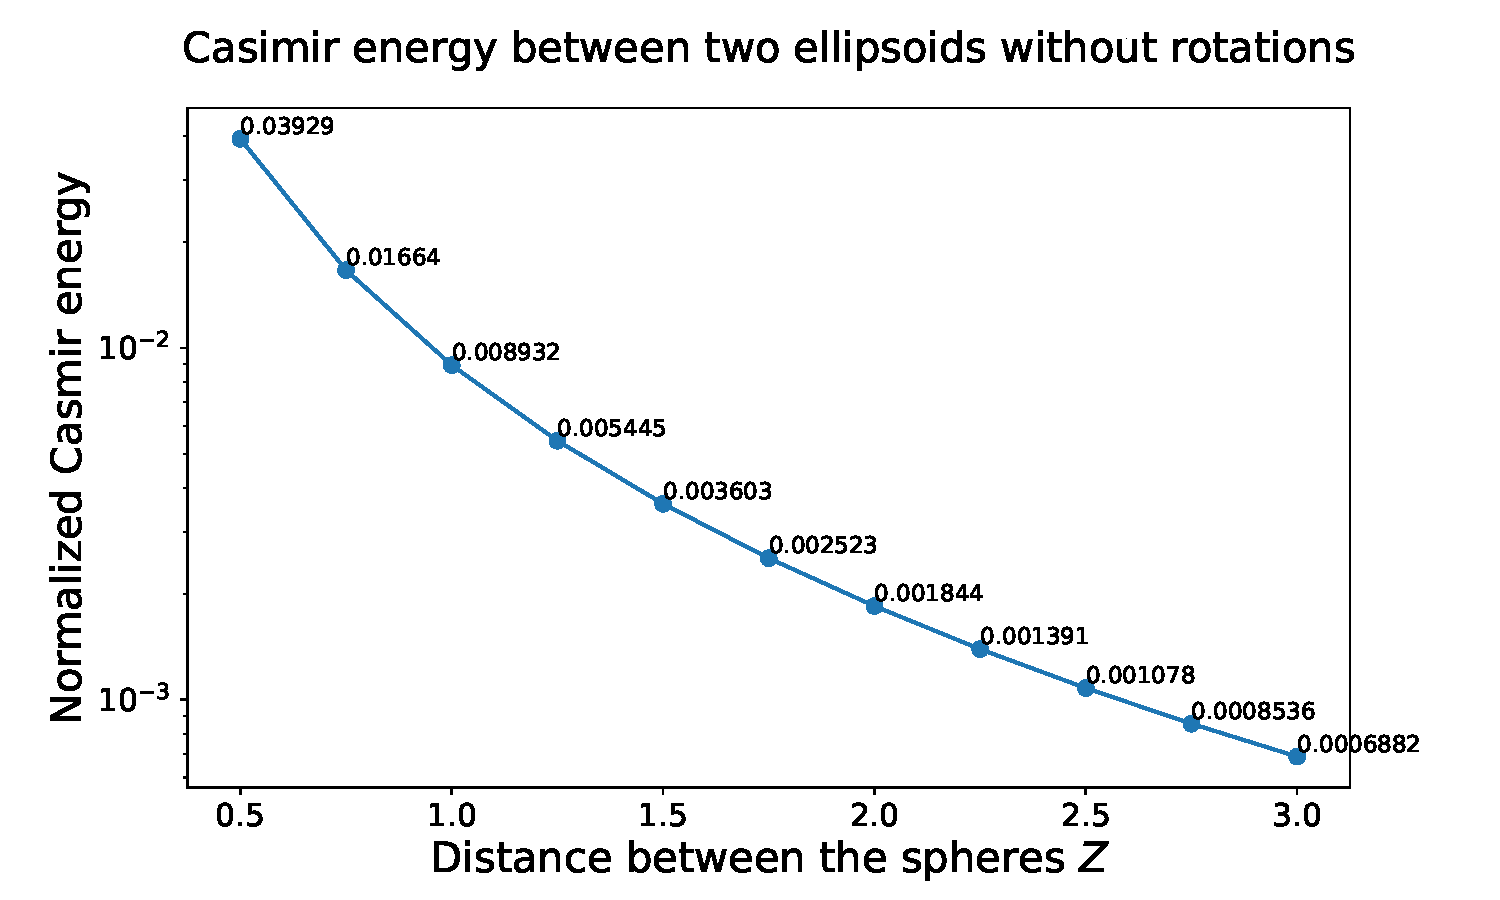
\includegraphics[scale = 0.5]{figures/CasE_ellipsoids.pdf}
            \caption{Casimir energy between two ellipsoids with different distances}
            \end{subfigure}\\[1ex]
    
        \begin{subfigure}{\linewidth}
        \centering
        \hspace*{-1cm}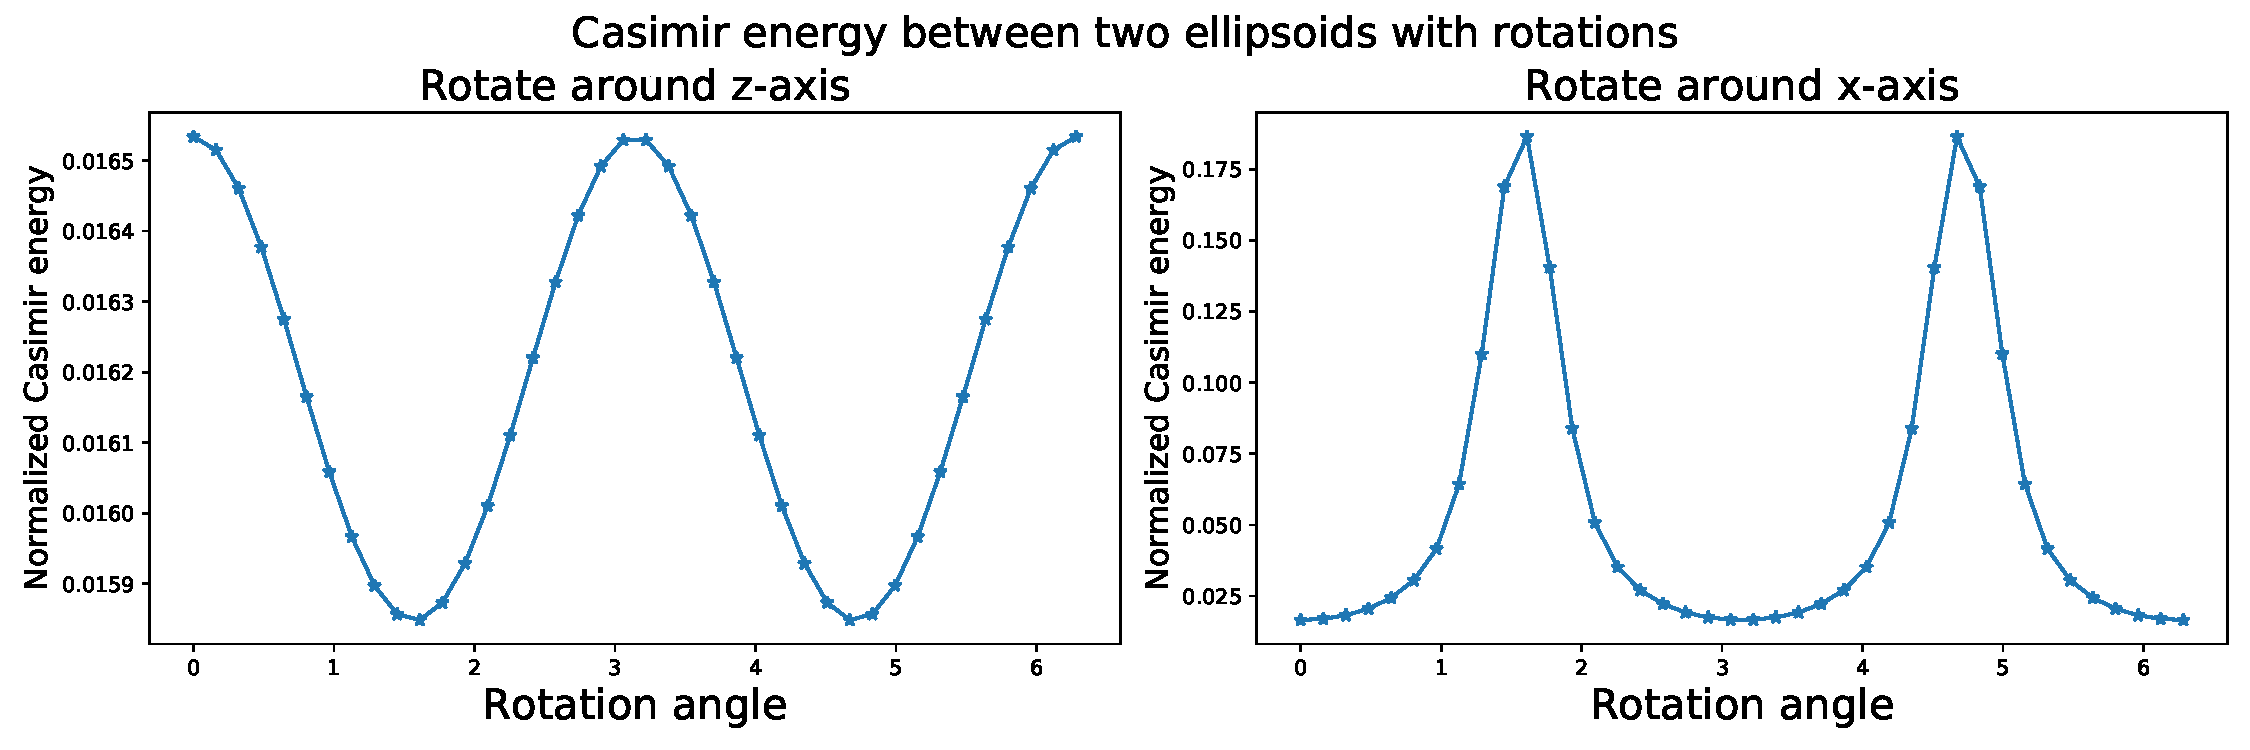
\includegraphics[scale = 0.5]{figures/CasE_ellipsoids_with_rotation.pdf}
        \caption{Casimir energy when one of the ellipsoids rotates}
        \end{subfigure}
        \caption{Two ellipsoids}
        \end{figure}

